\documentclass[twoside,12pt,a5paper]{article}
\usepackage[a5paper]{geometry}
\geometry{verbose,tmargin=2cm,bmargin=2cm,lmargin=2cm,rmargin=2cm}
\usepackage{fancyhdr}
\pagestyle{fancy}
\usepackage{lmodern}
\usepackage[utf8]{inputenc}
\usepackage[czech]{babel}	
\usepackage{epsfig}
\usepackage[chordbk]{sbmain}
\usepackage{multicol}
\cfoot{}
\usepackage{xkeyval}	% Inline todonotes
\usepackage[textsize = footnotesize]{todonotes}
\presetkeys{todonotes}{inline}{}

\title{KEYA zpěvník 2020 s notami}
\date{Verze: 1.2$\gamma$ (\today)}
%%%
% Redefine fonts from SongBook style
%%%
\font\myTinySF=cmss8 at 8pt
\renewcommand{\CpyRtInfoFont}{\tiny\myTinySF}

%%%
% Define fonts to use in the headers and footers of the songbook.
%%%
\newcommand{\LHeadFont}{\normalsize}            % = cmr12  at 12pt
\newcommand{\CHeadFont}{\normalsize}         % = cmr12  at 12pt
\newcommand{\RHeadFont}{\normalsize}            % = cmr12  at 12pt
\newcommand{\LFootFont}{\scriptsize}            % = cmr8   at  8pt
\newcommand{\CFootFont}{\tiny\myTinySF}         % = cmss8  at  8pt
\newcommand{\RFootFont}{\scriptsize}            % = cmr8   at  8pt

\fancyhead[LE,RO]{\CHeadFont{KEYA zpěvník 2020}}
\fancyhead[CE,CO]{\CHeadFont\thepage}

\begin{document}
\maketitle
\begin{center}


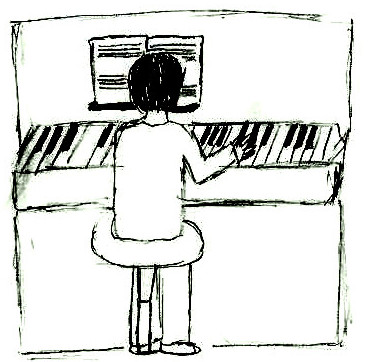
\includegraphics[width=0.8\textwidth]{pict/noty} 


\end{center}


\begin{center}



\includegraphics[width=0.4\textwidth]{pict/logo}


\end{center}
\cleardoublepage
\begin{multicols}{2}
\begin{footnotesize}
\tableofcontents{}
%\columnbreak%maybe
\end{footnotesize}
\end{multicols}
\clearpage
\section{Základní zpěvník}

\setcounter{page}{5}
\begin{song}{Amazonka}{A}{Hop Trop}
\includegraphics[width=\textwidth]{noty/a_amazonka}
\end{song}
\pagebreak

\setcounter{page}{8}
\begin{song}{Batalion}{C}{Spirituál Kvintet}
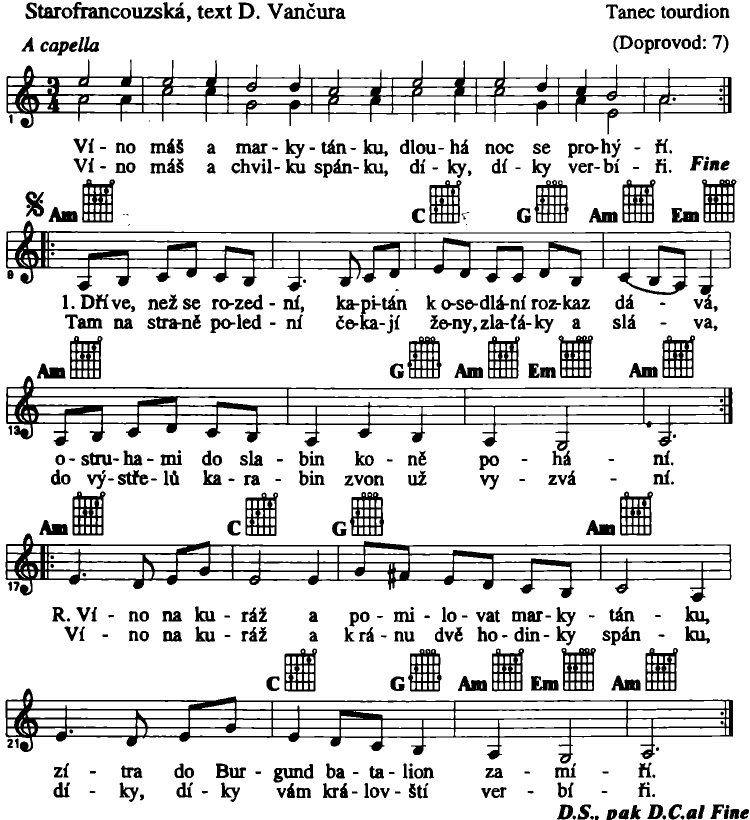
\includegraphics[width=\textwidth]{noty/a_batalion} \end{song} \pagebreak

\setcounter{page}{9}
\begin{song}{Bedna od whisky}{C}{Miki Ryvola}
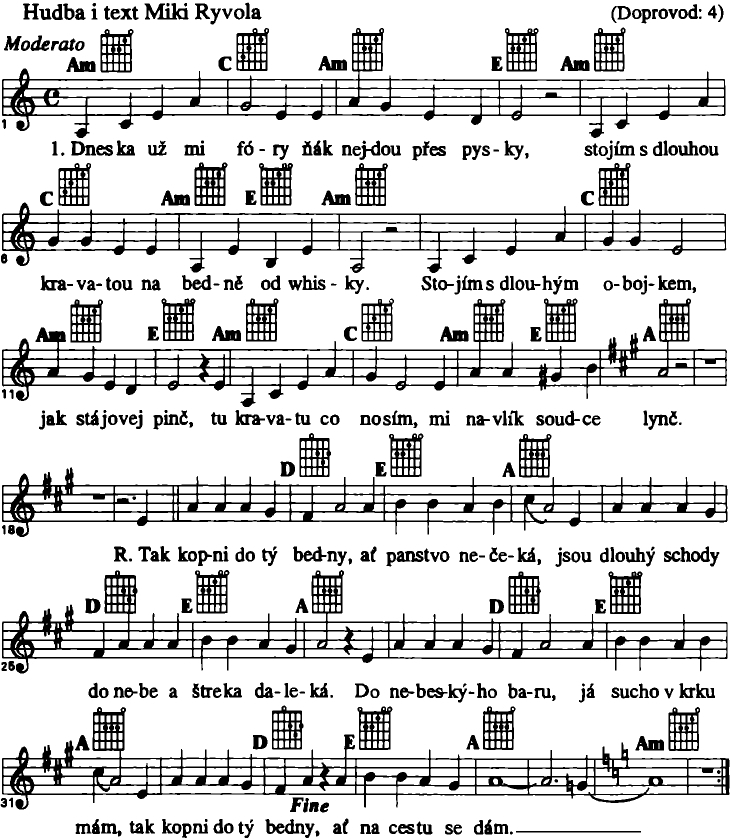
\includegraphics[width=\textwidth]{noty/a_bedna-od-whisky} \end{song} \pagebreak

\setcounter{page}{10}
\begin{song}{Bláznova ukolébavka}{D}{Lunetic}
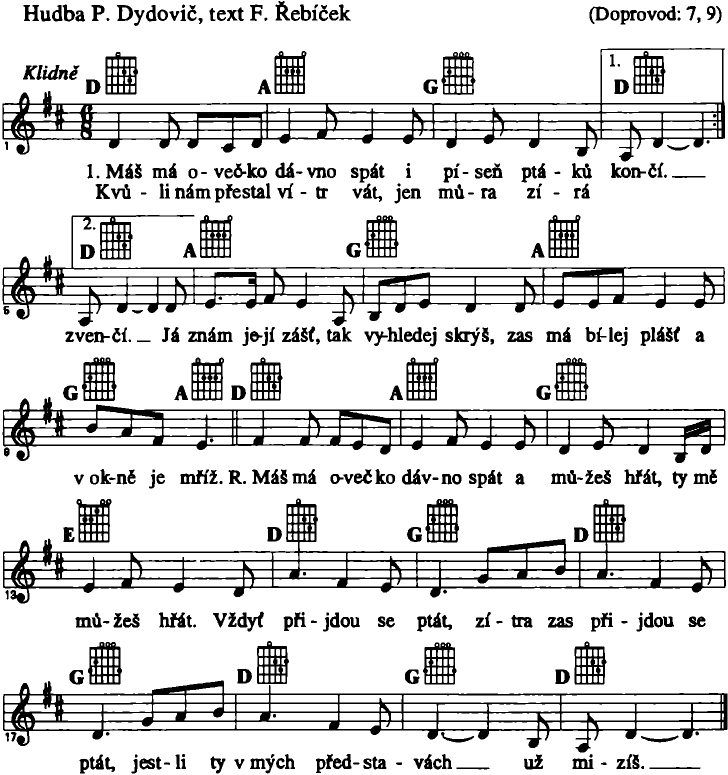
\includegraphics[width=\textwidth]{noty/a_bláznova-ukolébavka} \end{song} \pagebreak

\setcounter{page}{11}
\begin{song}{Bratříčku, zavírej vrátka}{G}{Karel Kryl}
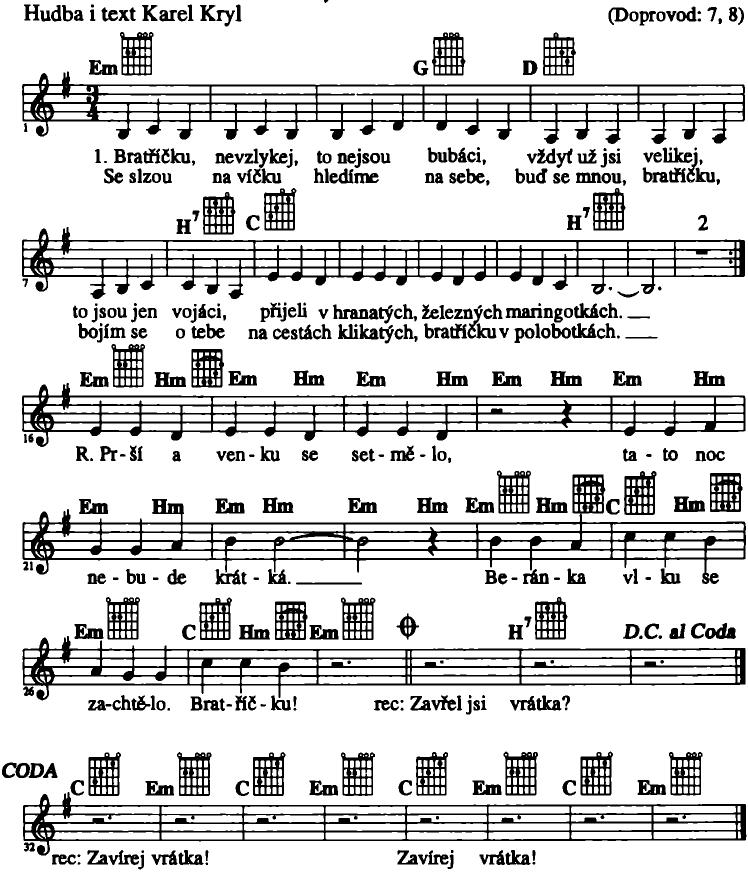
\includegraphics[width=\textwidth]{noty/a_bratříčku-zavírej-vrátka} \end{song} \pagebreak

\setcounter{page}{12}
\begin{song}{Čarodějnice z Amesbury}{F}{Asonance}
\begin{center}
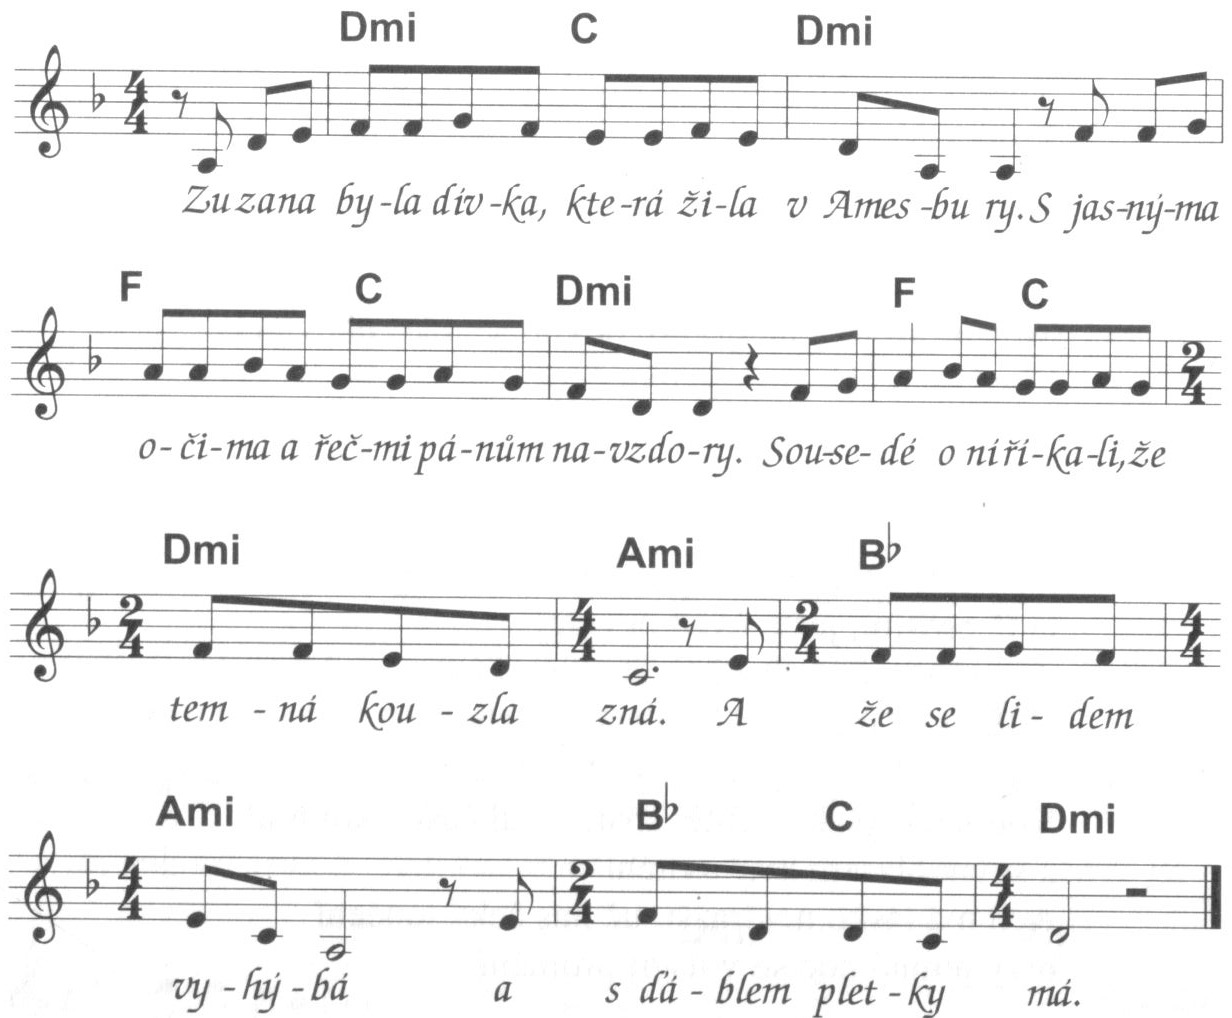
\includegraphics[width=0.77\textwidth]{noty/a_carodejnice1} 

\;

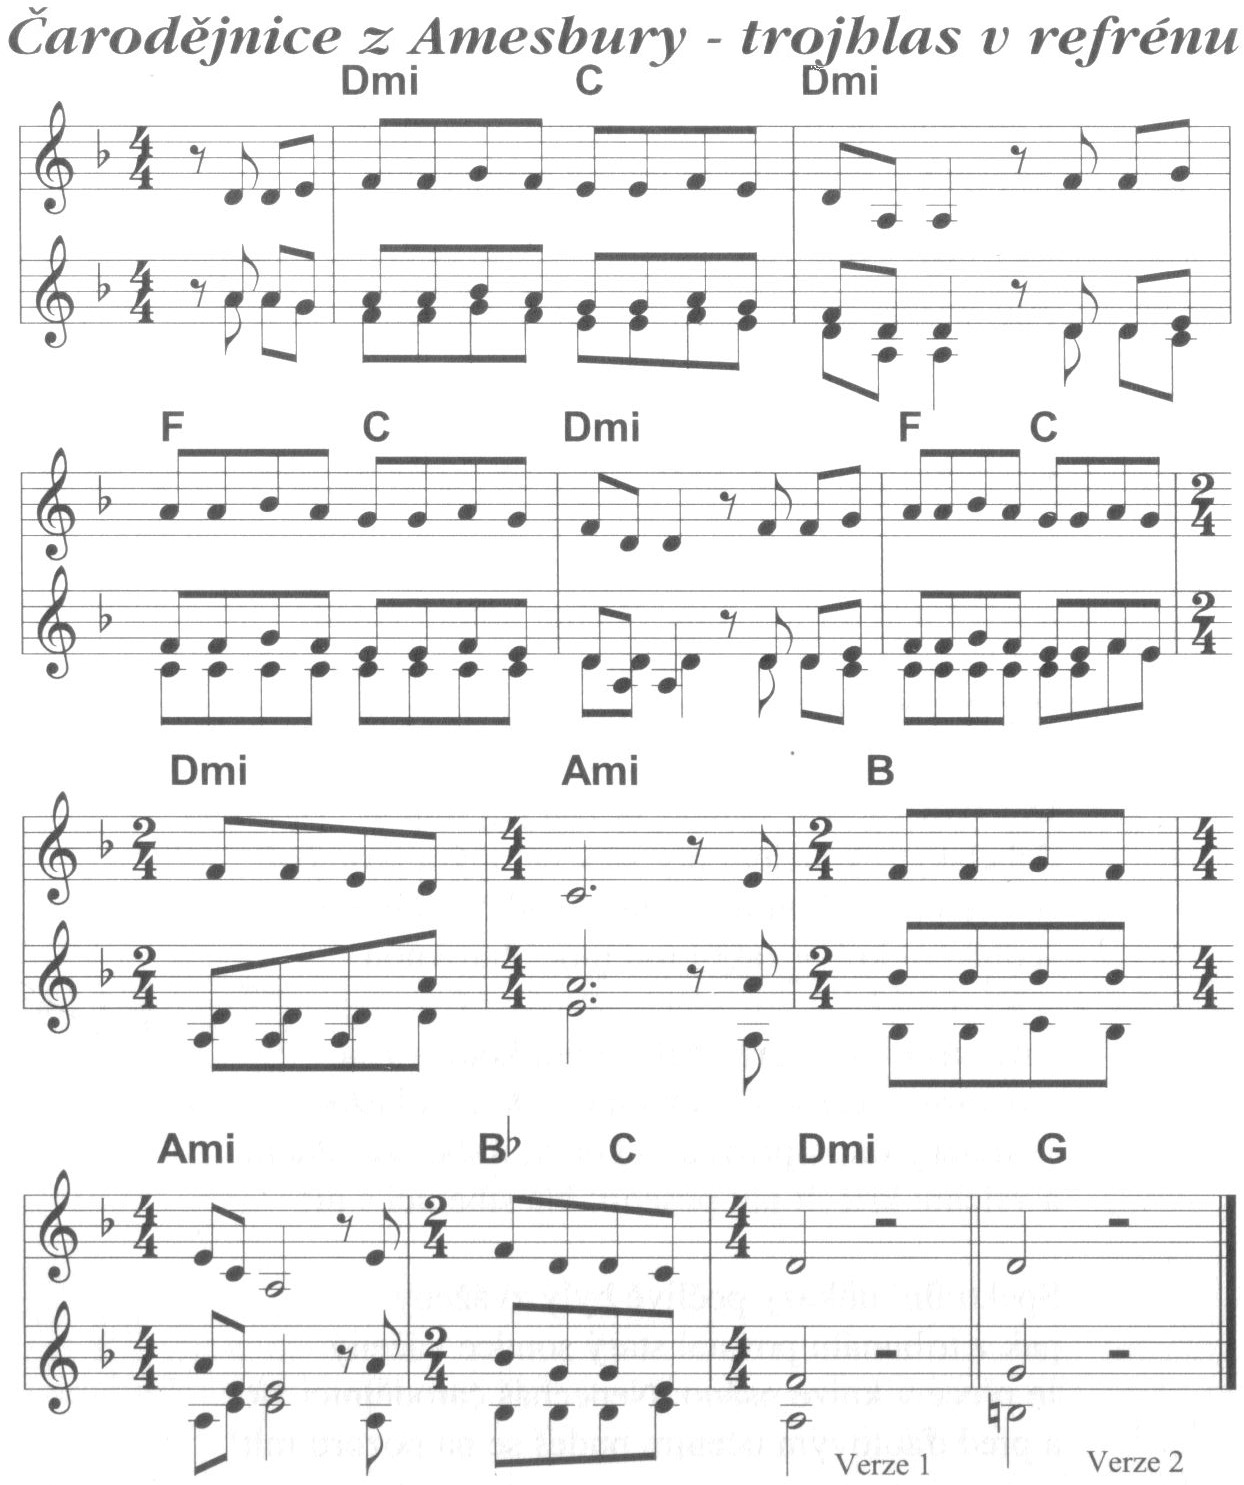
\includegraphics[width=0.77\textwidth]{noty/a_carodejnice2} 
 
\end{center} 
\end{song} \pagebreak

\setcounter{page}{15}
\begin{song}{Černá díra}{G}{Karel Plíhal}
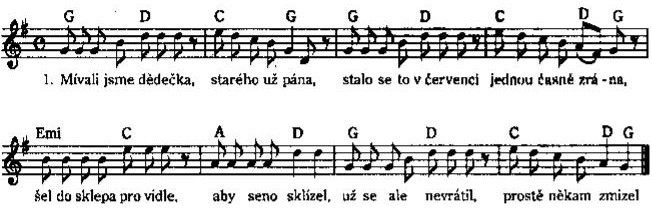
\includegraphics[width=\textwidth]{noty/a_czerná-díra} \end{song} \pagebreak

\setcounter{page}{18}
\begin{song}{Darmodej}{C}{Jaromír Nohavica}
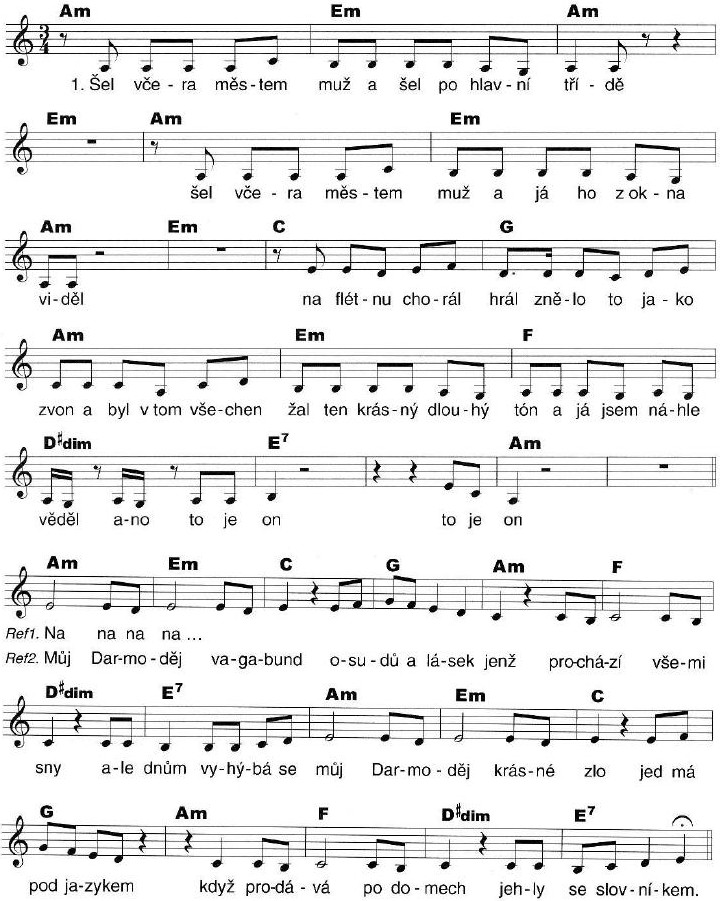
\includegraphics[width=\textwidth]{noty/a_darmoděj} \end{song} \pagebreak

\setcounter{page}{19}
\begin{song}{Dej mi víc své lásky}{G}{Olympic}
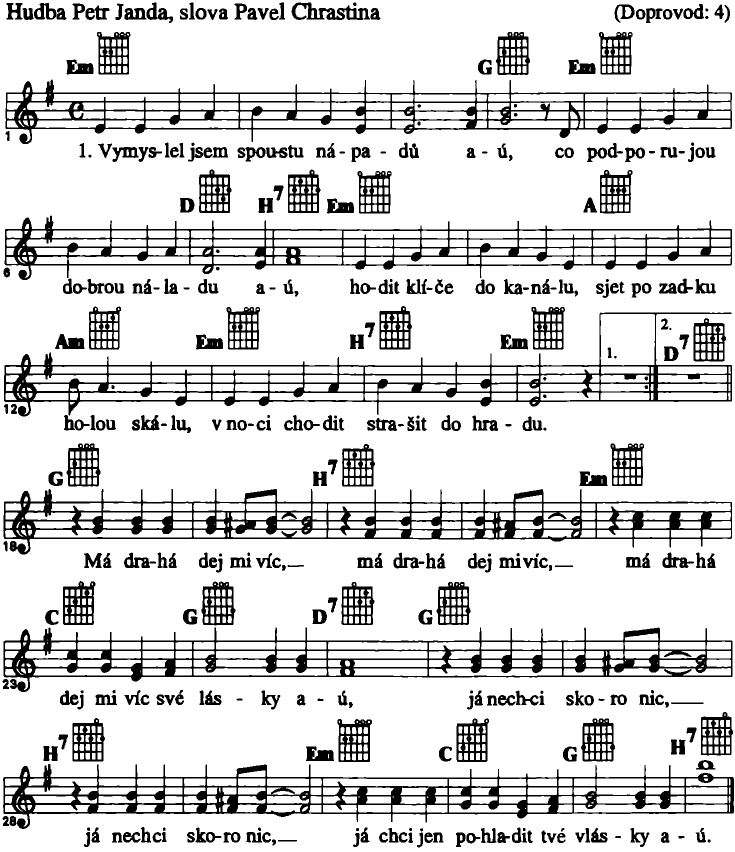
\includegraphics[width=\textwidth]{noty/a_dej-mi-víc-své-lásky} \end{song} \pagebreak

\setcounter{page}{21}
\begin{song}{Divoké koně}{C}{Jaromír Nohavica}
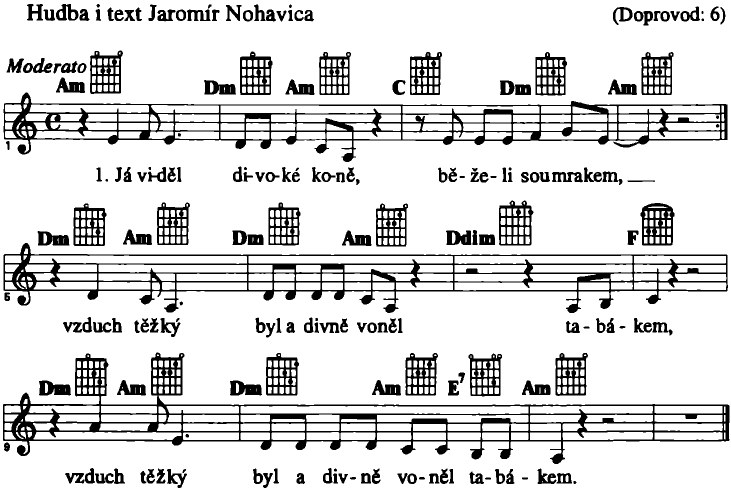
\includegraphics[width=\textwidth]{noty/a_divoké-koně} \end{song} \pagebreak

\setcounter{page}{22}
\begin{song}{Donald MacGillavry}{G}{Asonance}
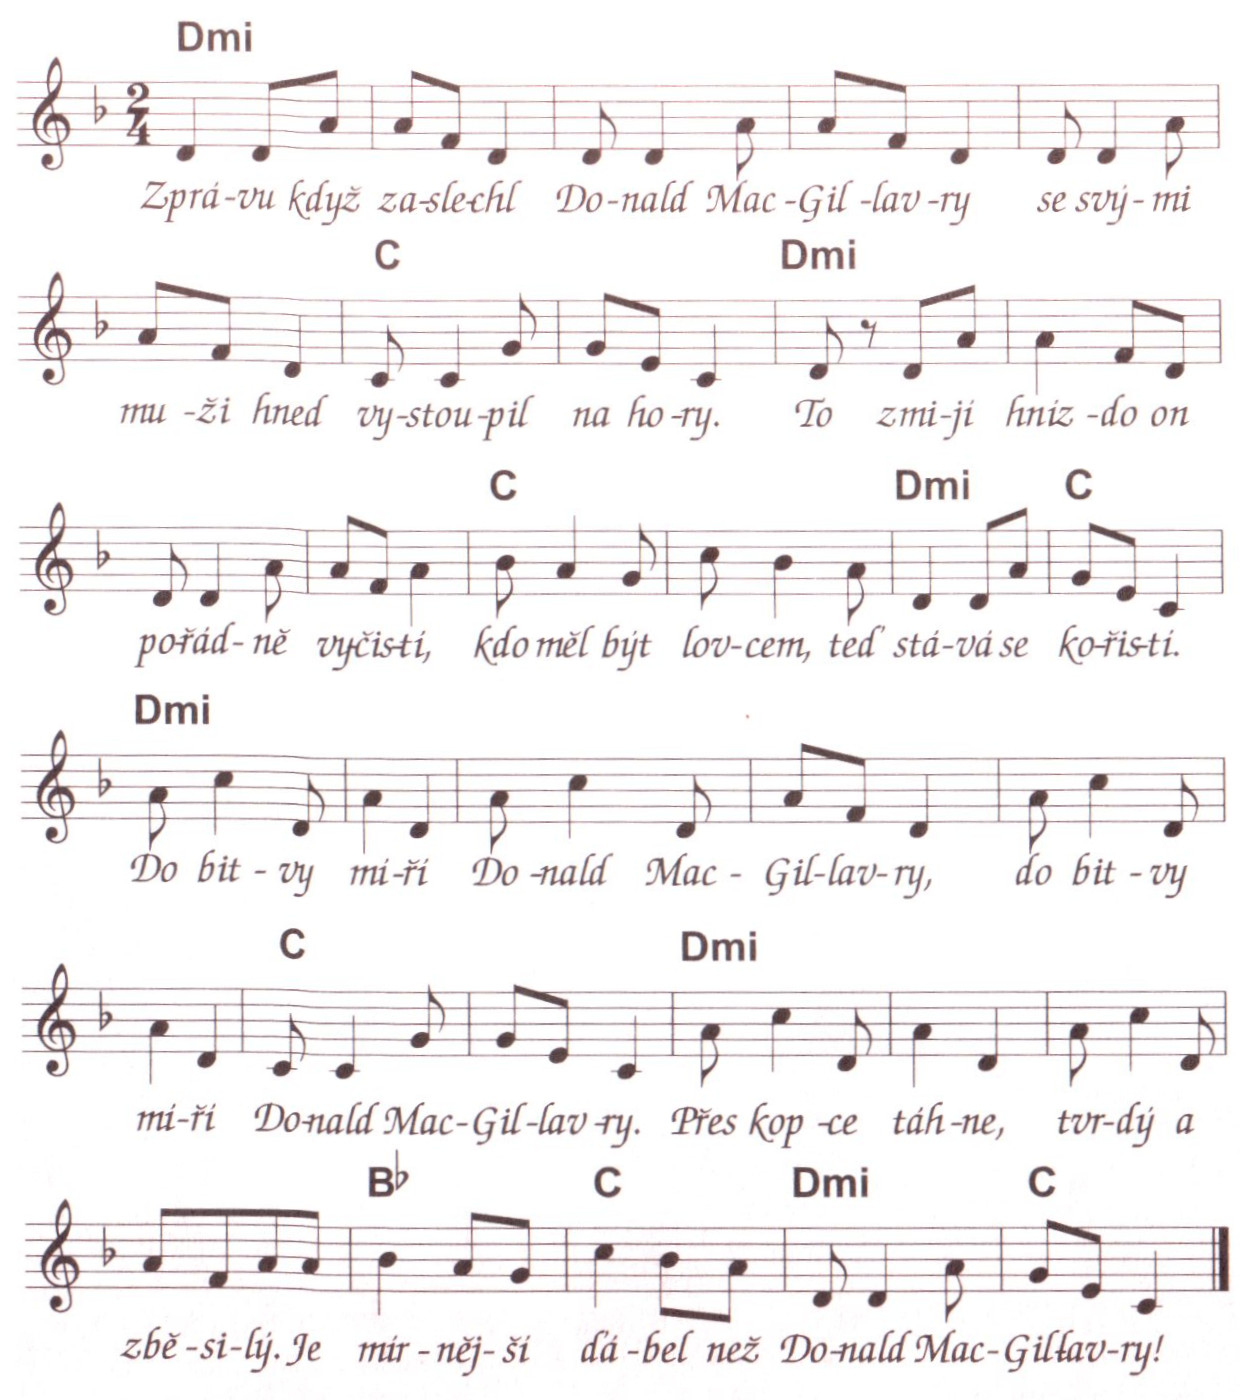
\includegraphics[width=0.72\textwidth]{noty/a_donald-macgallavry-1}\\
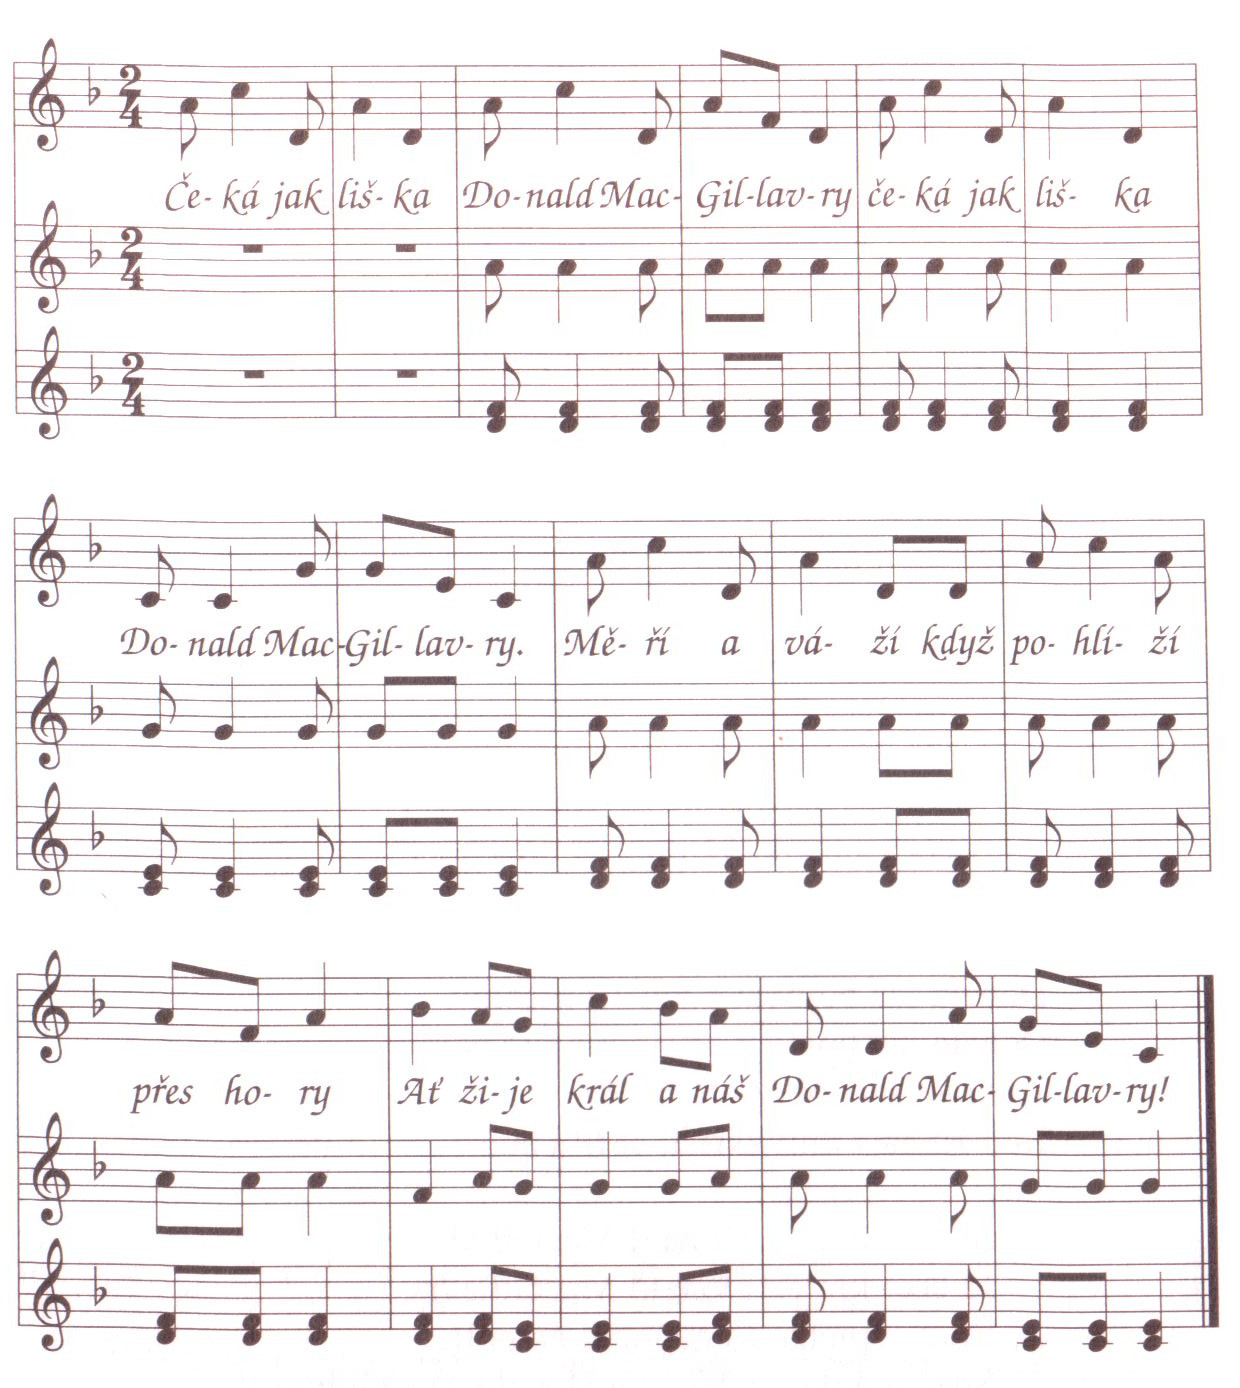
\includegraphics[width=0.75\textwidth]{noty/a_donald-macgallavry-2} \end{song} \pagebreak

\setcounter{page}{23}
\begin{song}{Dva Havrani}{F}{Asonance}
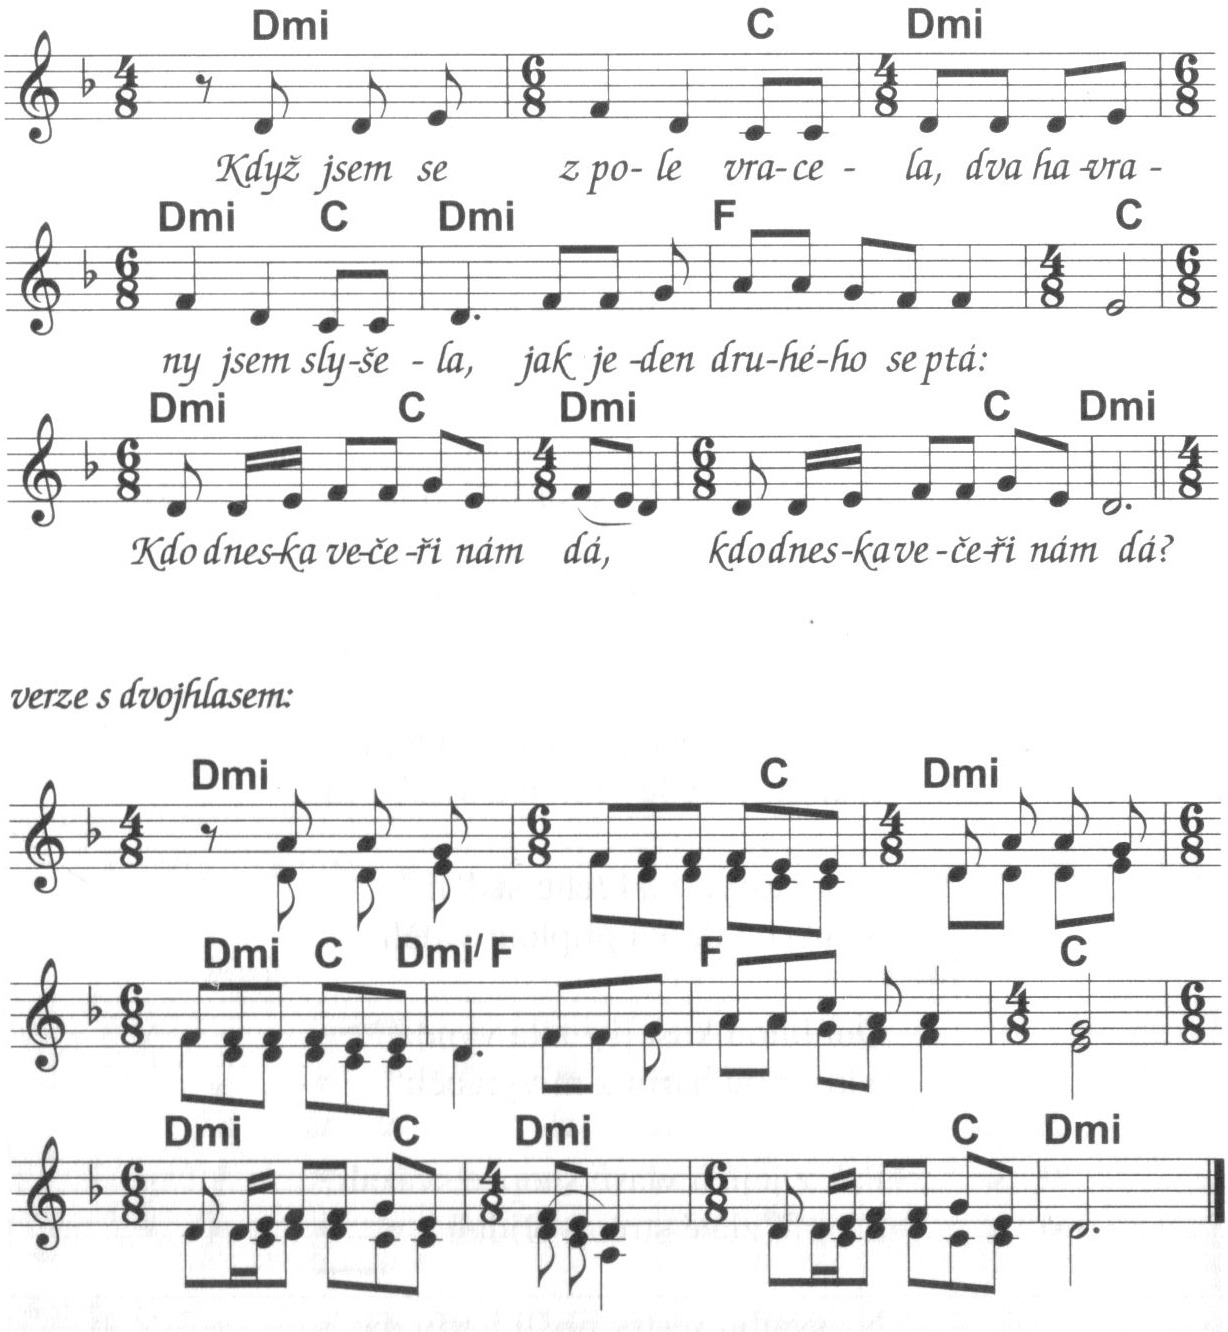
\includegraphics[width=\textwidth]{noty/a_dva-havrani} \end{song} \pagebreak

\setcounter{page}{24}
\begin{song}{Fi-li-mi}{As}{Spiritual kvintet}
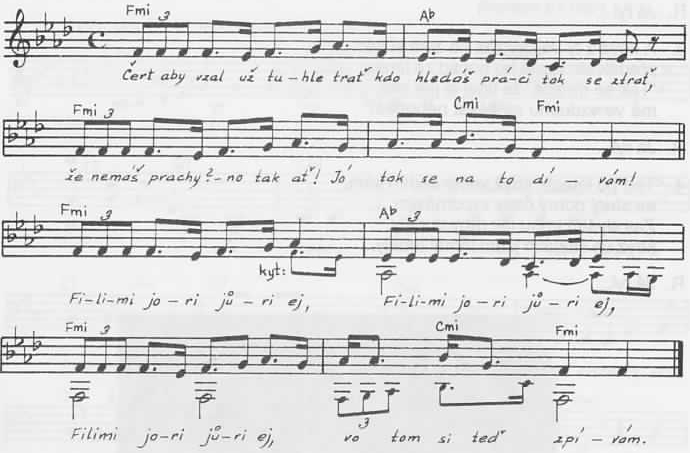
\includegraphics[width=\textwidth]{noty/a_fi-li-mi} \end{song} \pagebreak

\input{noty/a_frankie-dlouhán.tex}
\setcounter{page}{26}
\begin{song}{Hlídač krav}{D}{Jaromír Nohavica}
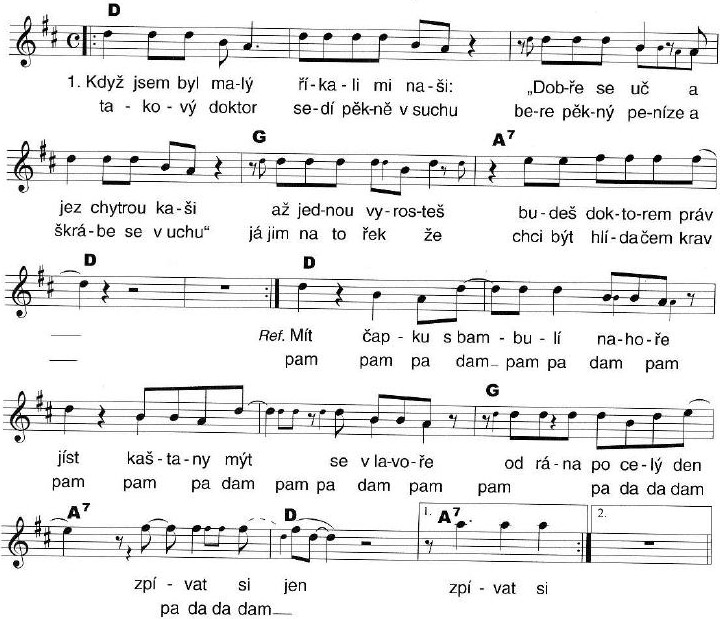
\includegraphics[width=\textwidth]{noty/a_hlídač-krav} \end{song} \pagebreak

\setcounter{page}{27}
\begin{song}{Ho ho Watanay}{G}{Pavel Lohonka Žalman}
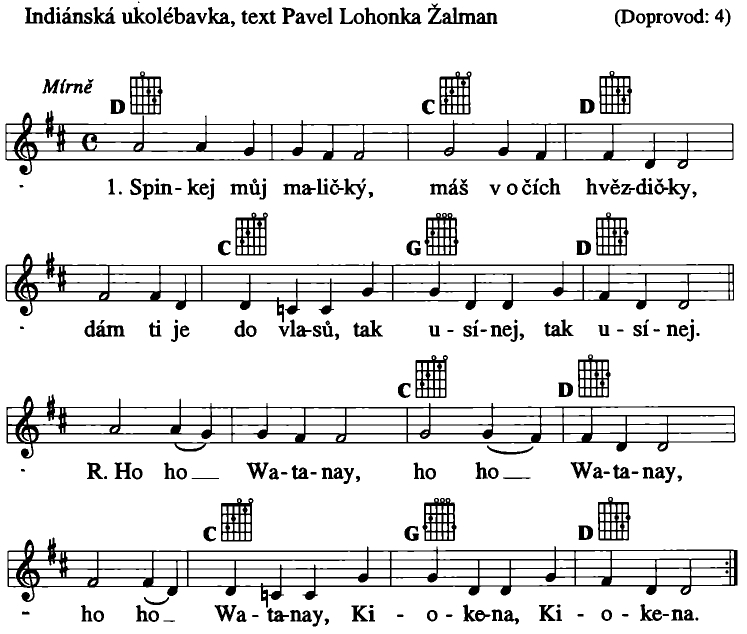
\includegraphics[width=\textwidth]{noty/a_ho-ho-watanay} \end{song} \pagebreak

\setcounter{page}{28}
\begin{song}{Hospoda U Davida}{G}{Fleret}
\begin{center}
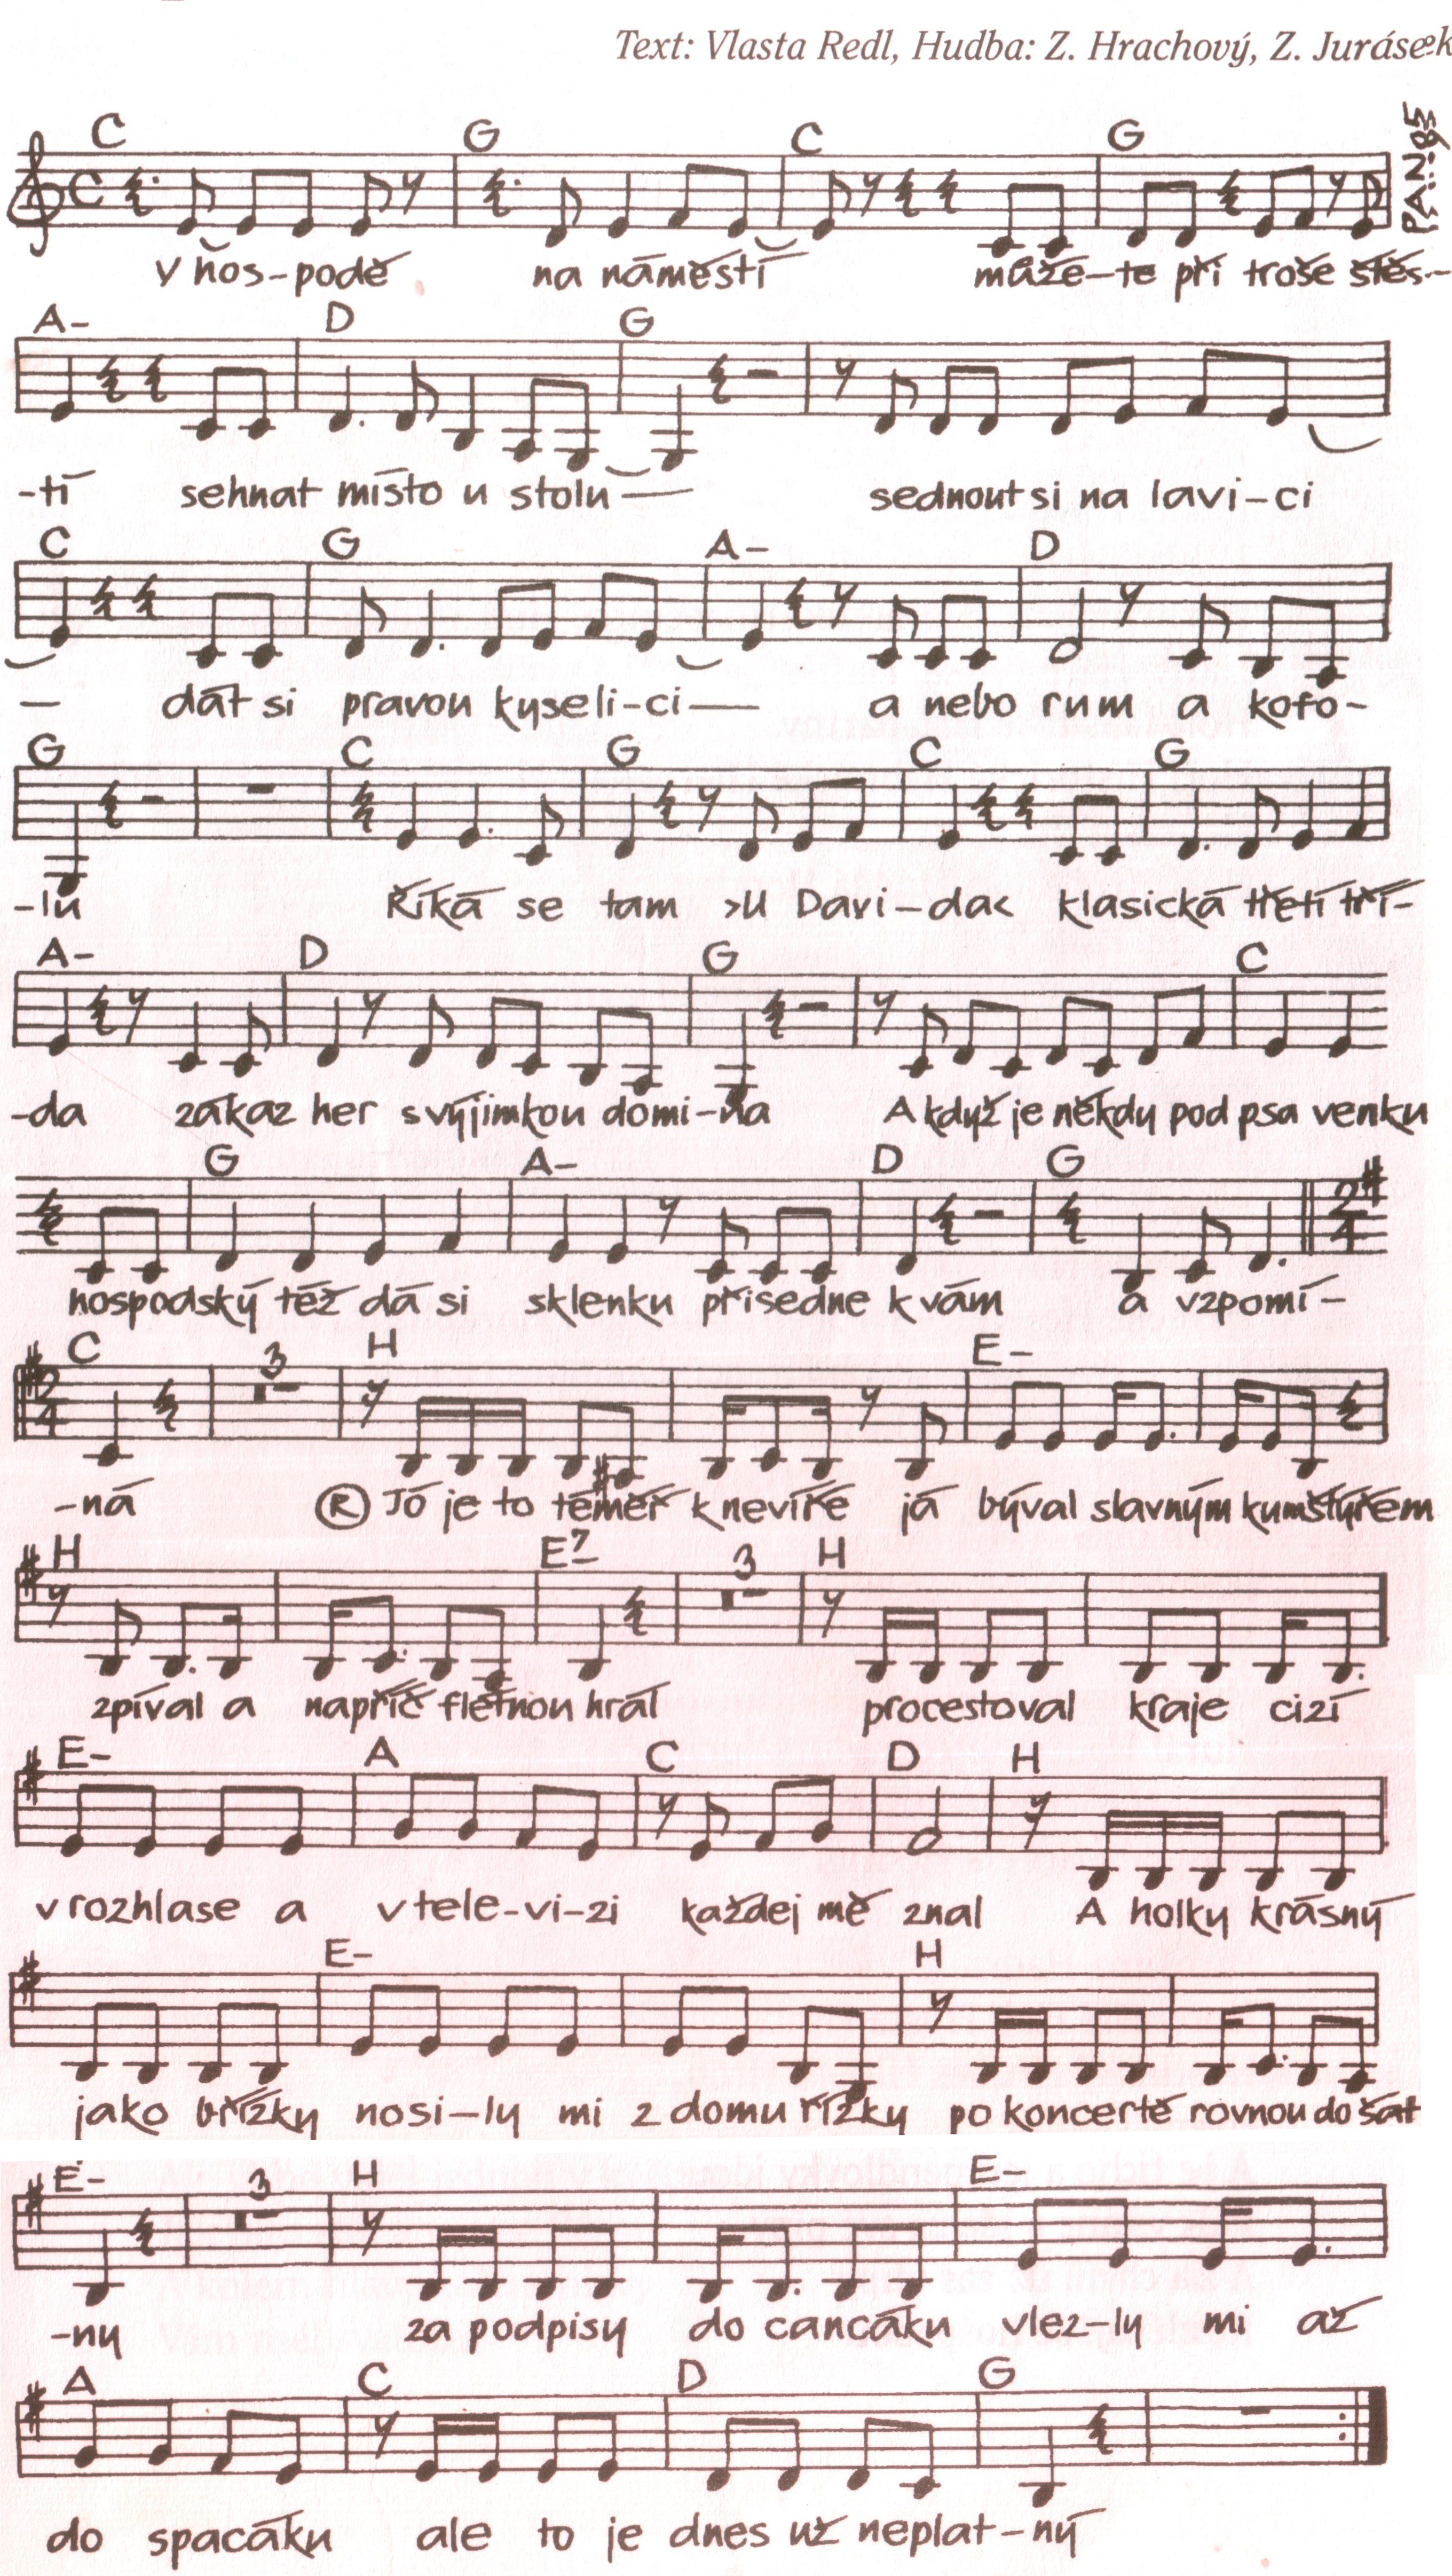
\includegraphics[width=0.9\textwidth]{noty/a_hospoda-u-davida}
\end{center}
\end{song}
\pagebreak

\setcounter{page}{30}
\begin{song}{Hrobař}{G}{Premier}
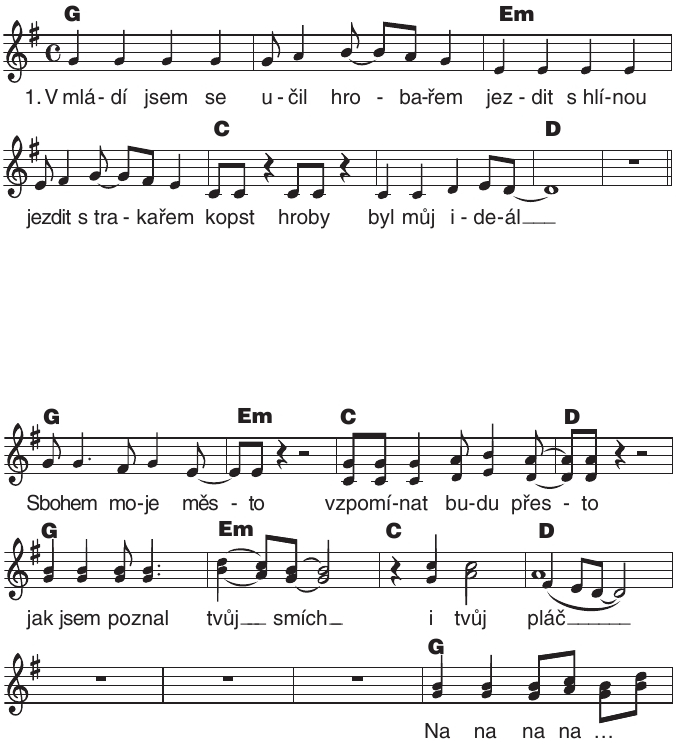
\includegraphics[width=\textwidth]{noty/a_hrobař} \end{song} \pagebreak

\setcounter{page}{32}
\begin{song}{Hučka}{G}{Zelenáči}
\begin{center}
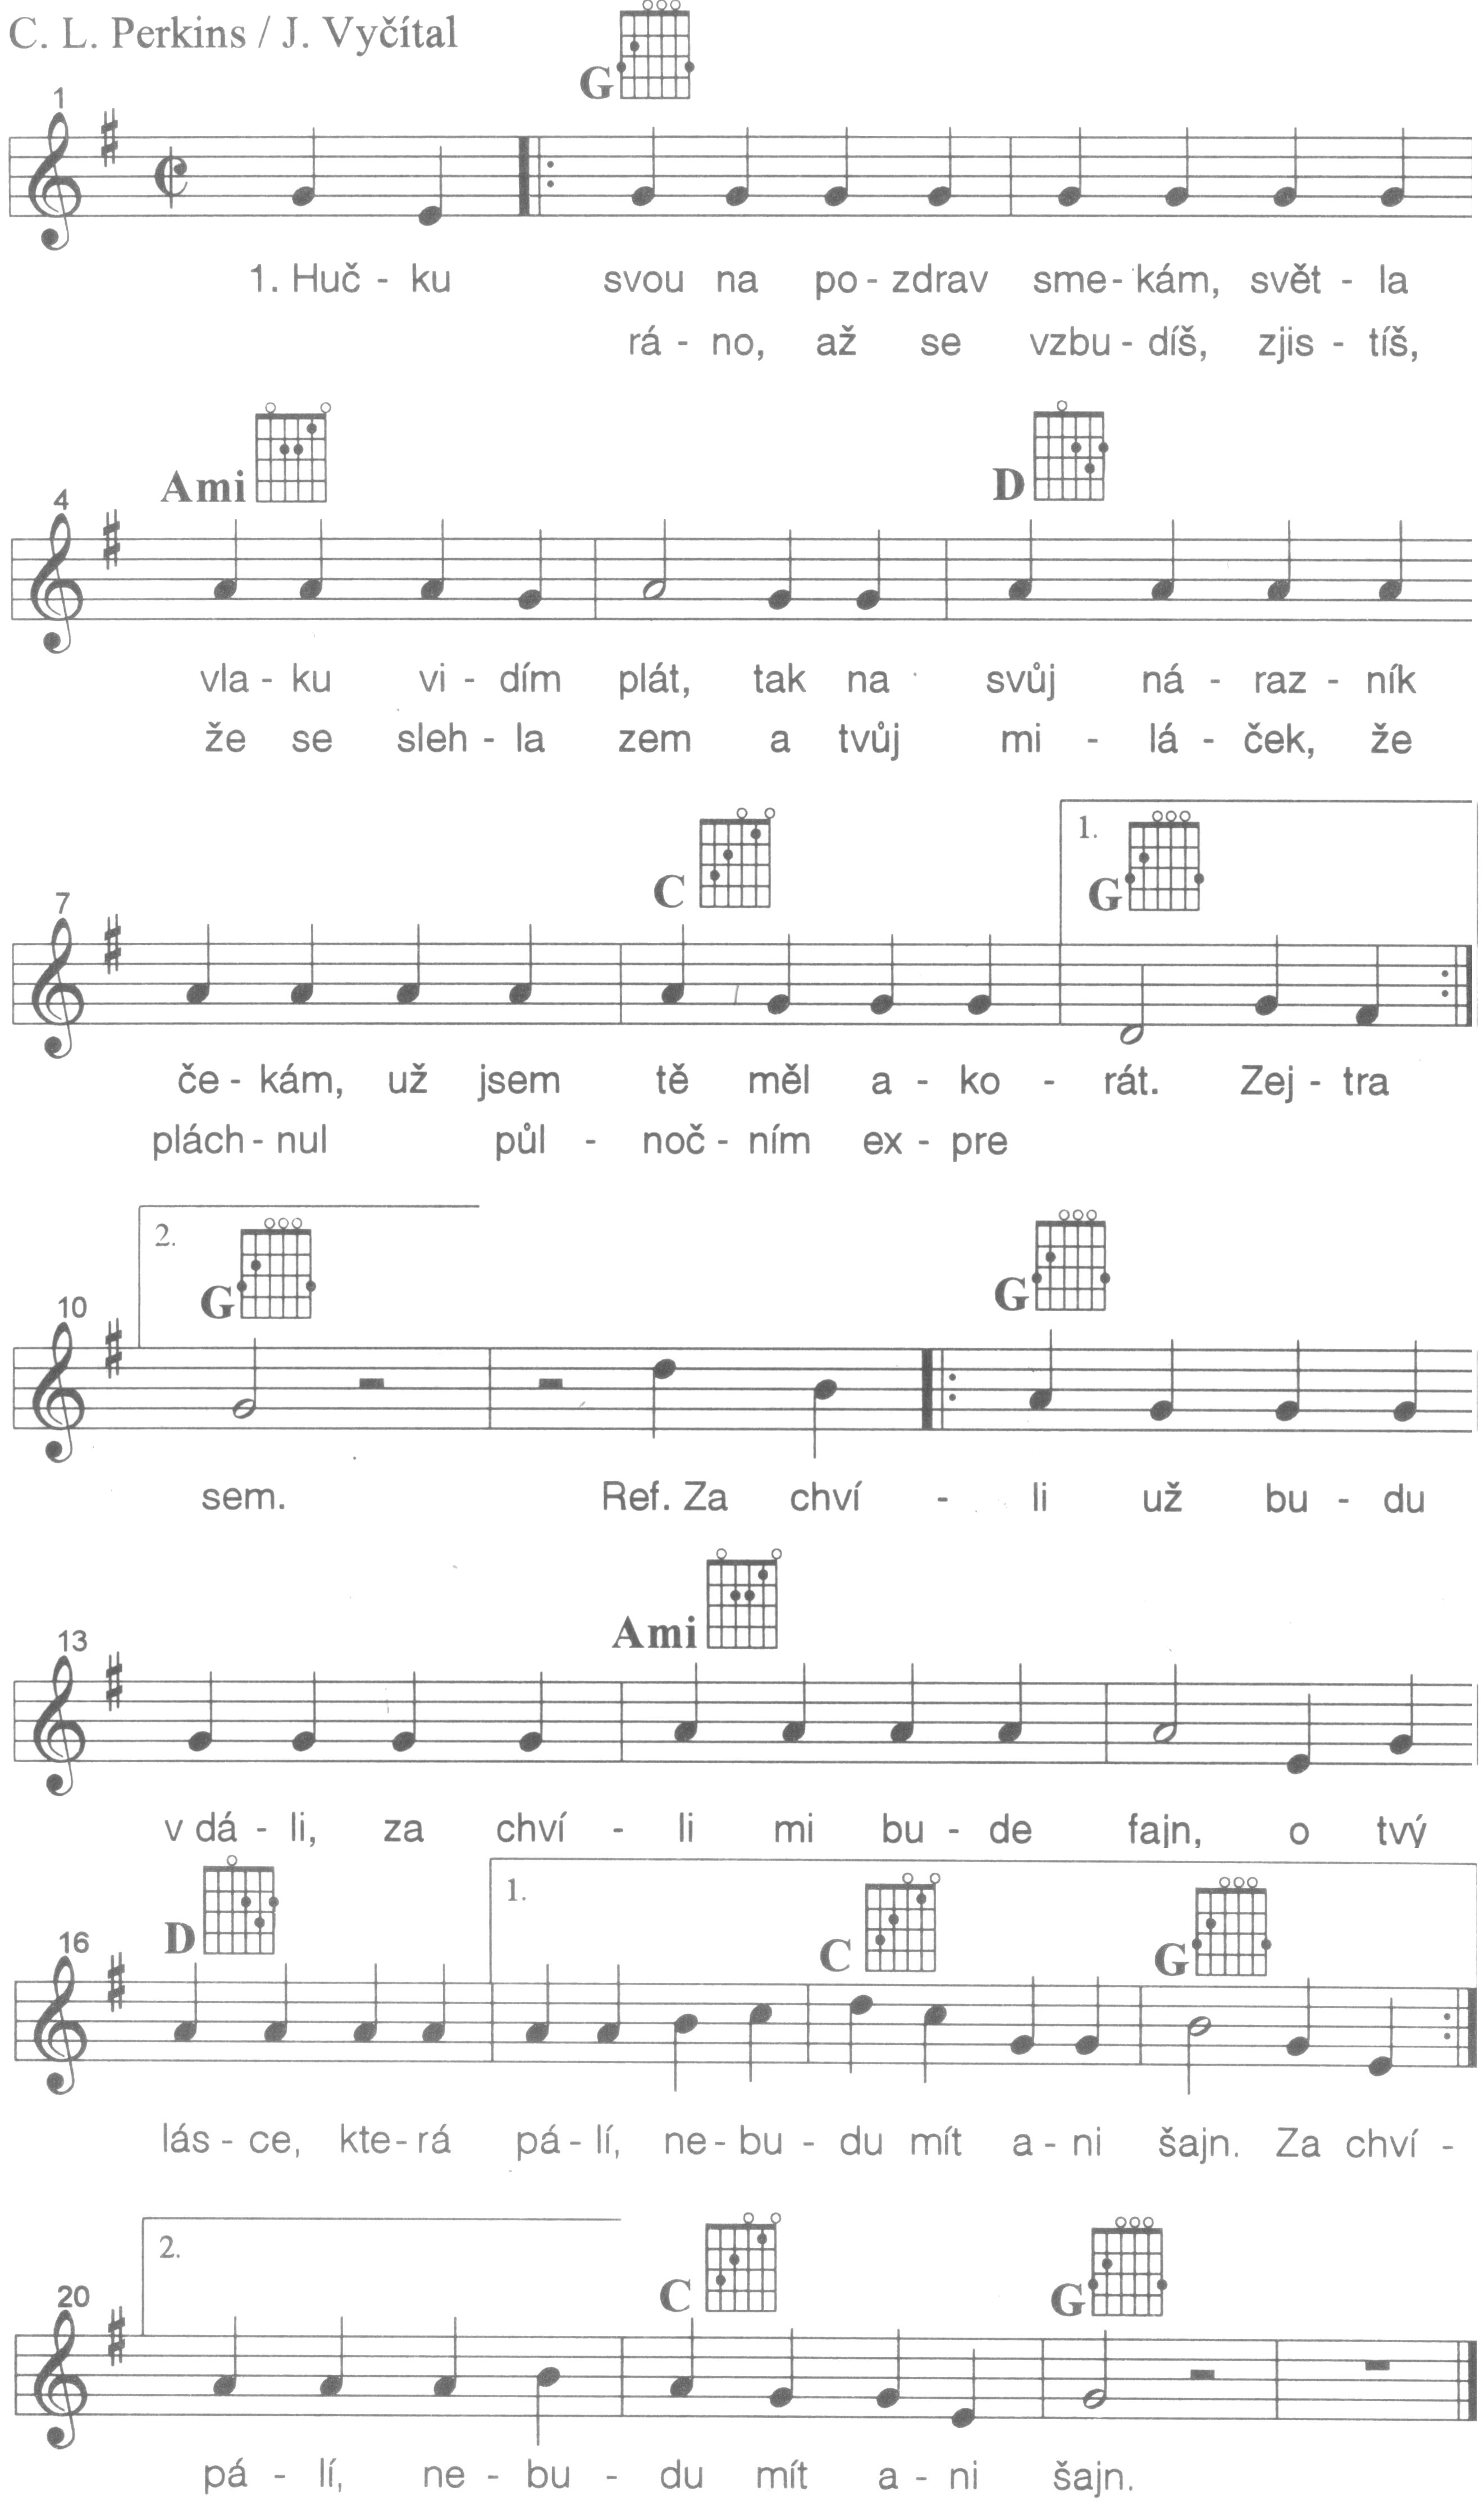
\includegraphics[height=0.9\textheight]{noty/a_hučka} 
\end{center}
\end{song} \pagebreak

\setcounter{page}{33}
\begin{song}{Hudsonský šífy}{C}{Wabi Daněk}
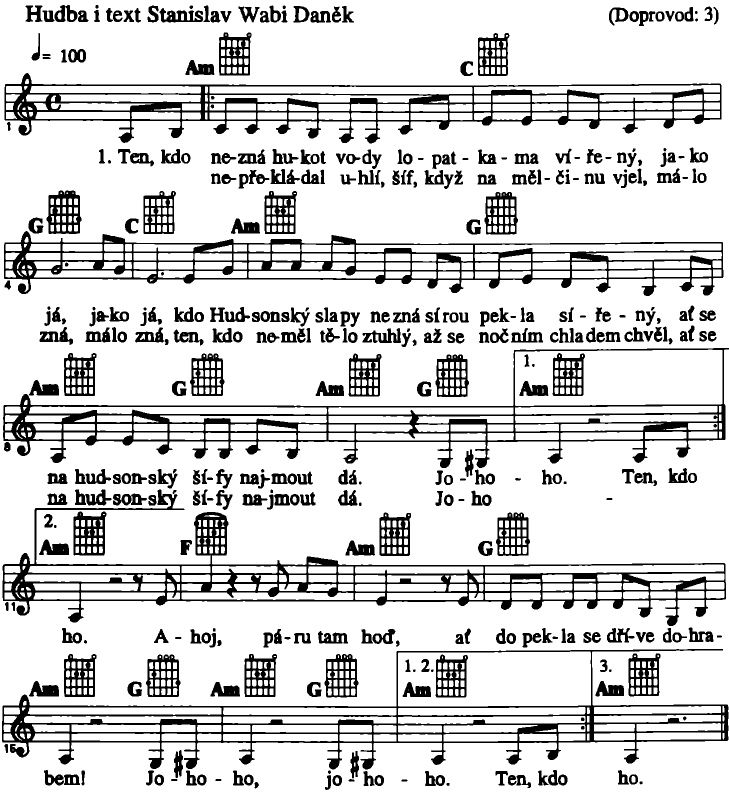
\includegraphics[width=\textwidth]{noty/a_hudsonský-šífy} \end{song} \pagebreak

\setcounter{page}{34}
\begin{song}{Jarní kurýr}{C}{Miki Ryvola}
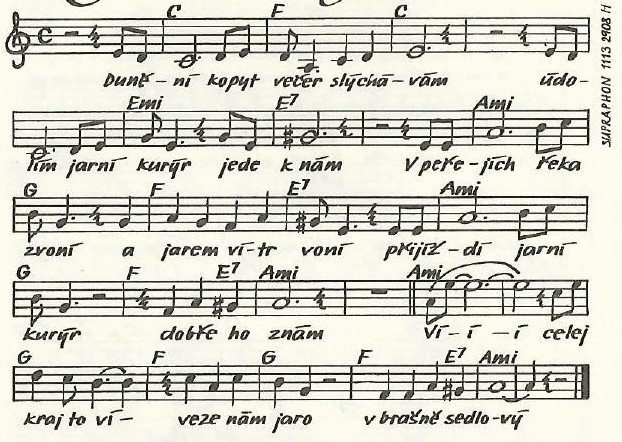
\includegraphics[width=\textwidth]{noty/a_jarní-kurýr} \end{song} \pagebreak

\setcounter{page}{35}
\begin{song}{Jarní tání}{C}{Jan Nedvěd}
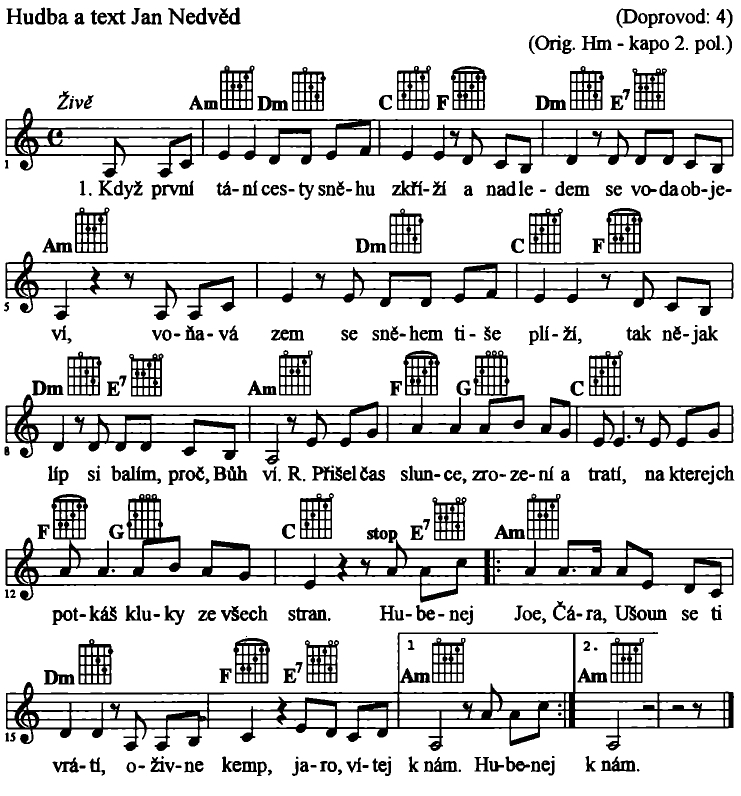
\includegraphics[width=\textwidth]{noty/a_jarní-tání} \end{song} \pagebreak

\setcounter{page}{36}
\begin{song}{Jaro}{C}{}
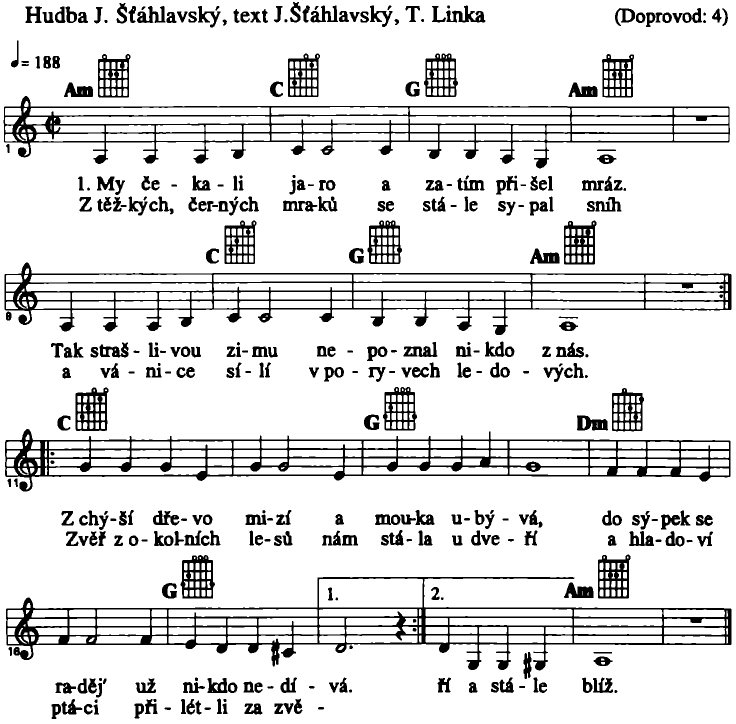
\includegraphics[width=\textwidth]{noty/a_jaro} \end{song} \pagebreak

\input{noty/a_jasný-jak-facka.tex}
\setcounter{page}{38}
\begin{song}{Já s tebou žít nebudu}{G}{Nerez}
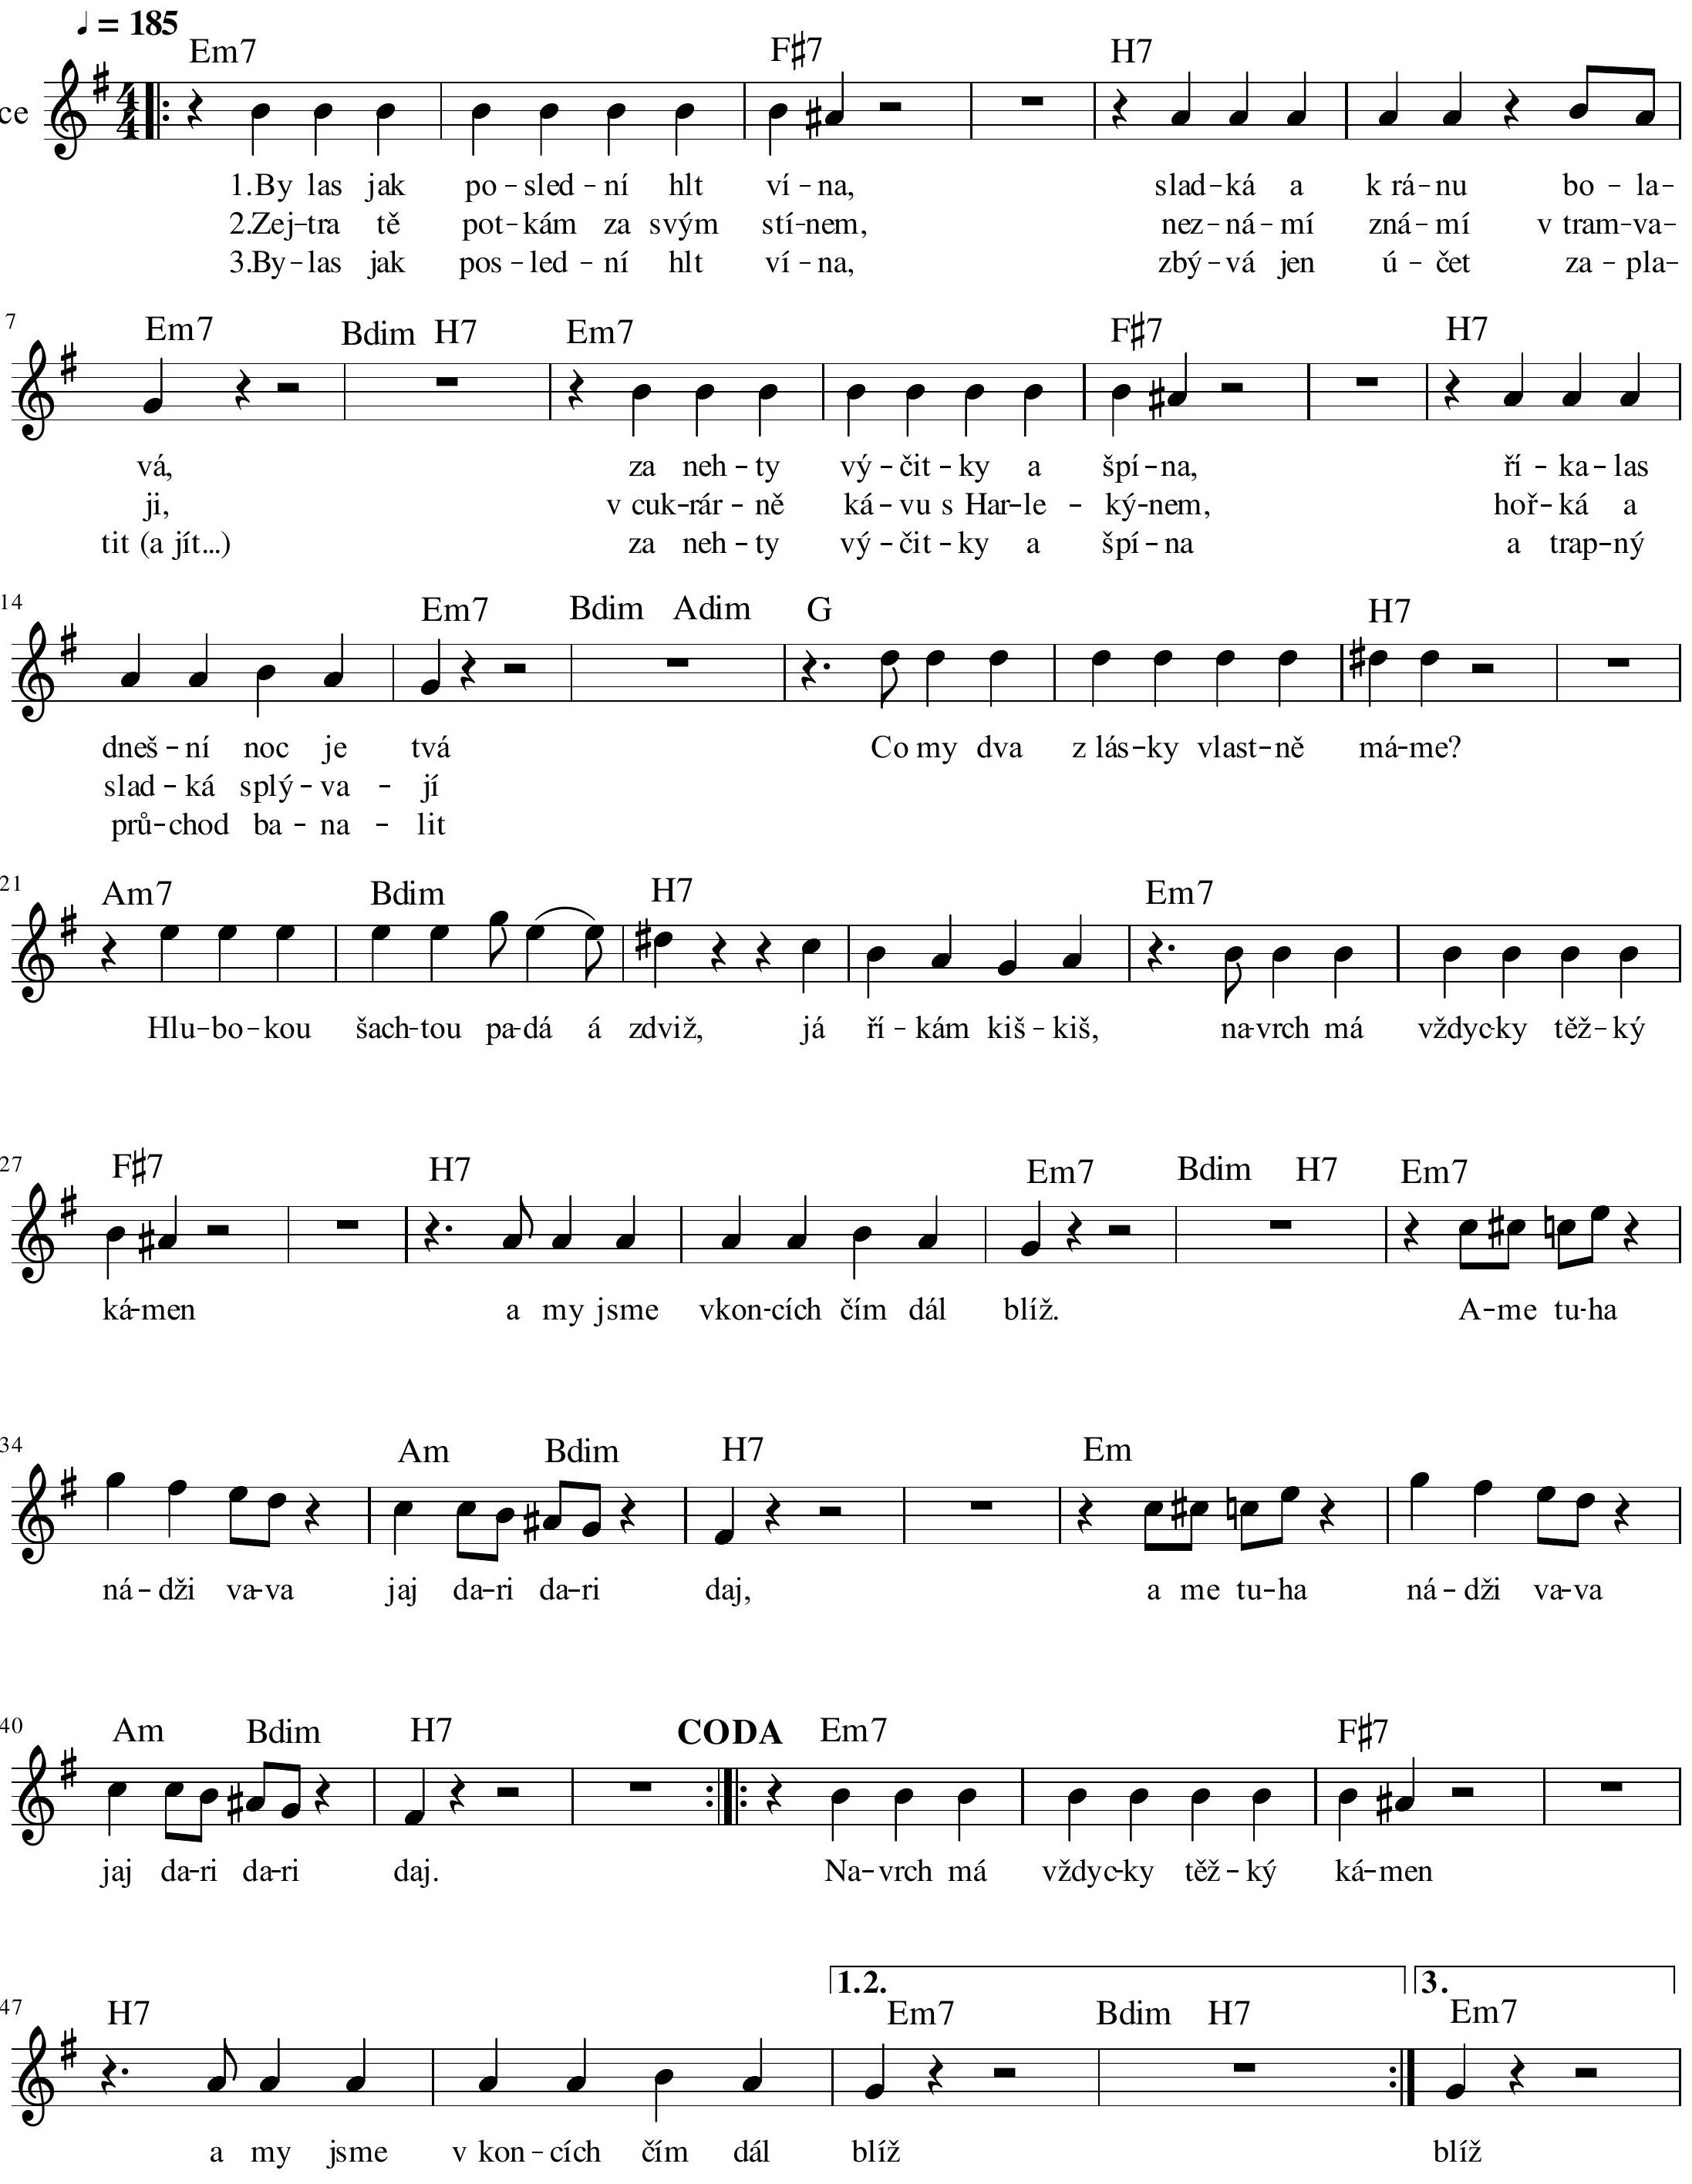
\includegraphics[width=\textwidth]{noty/a_já-s-tebou-žít-nebudu} \end{song} \pagebreak

\setcounter{page}{39}
\begin{song}{Jdem zpátky do lesů}{G}{Pavel Lohonka Žalman}
\begin{center}
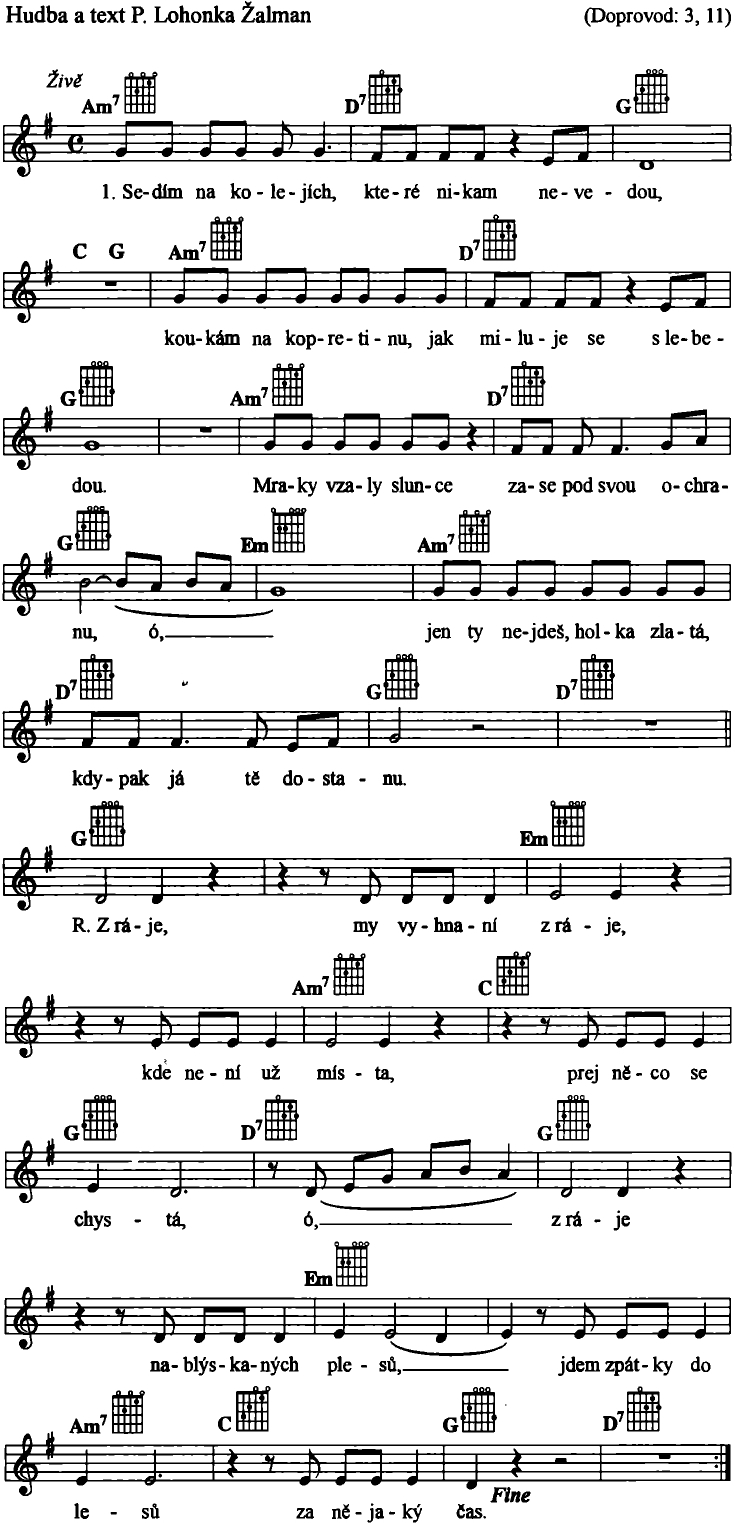
\includegraphics[width=0.8\textwidth]{noty/a_jdem-zpátky-do-lesů} 
\end{center}
\end{song} \pagebreak

\setcounter{page}{40}
\begin{song}{Jdou po mě jdou}{D}{Jaromír Novavica}
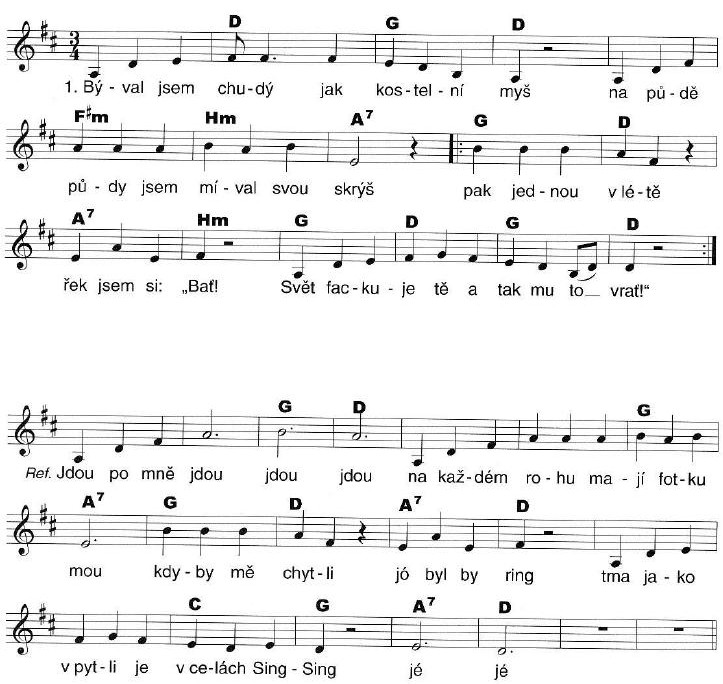
\includegraphics[width=\textwidth]{noty/a_jdou-po-mě-jdou} \end{song} \pagebreak

\setcounter{page}{41}
\begin{song}{Když mě brali za vojáka}{C}{Jaromír Nohavica}
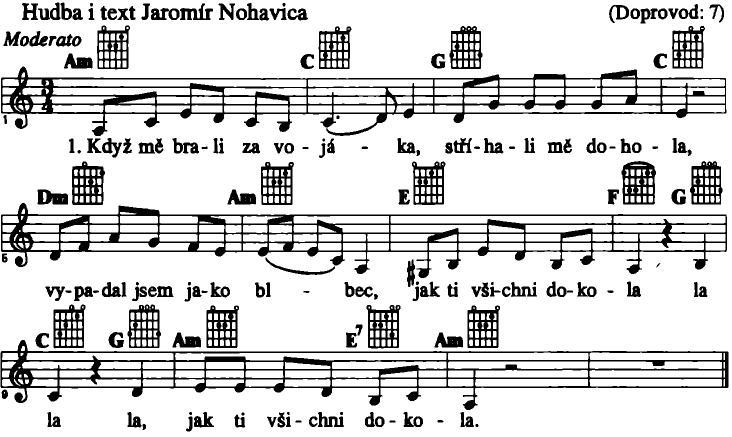
\includegraphics[width=\textwidth]{noty/a_když-mě-brali-za-vojáka} \end{song} \pagebreak

\setcounter{page}{42}
\begin{song}{Kluziště}{C}{Karel Plíhal}
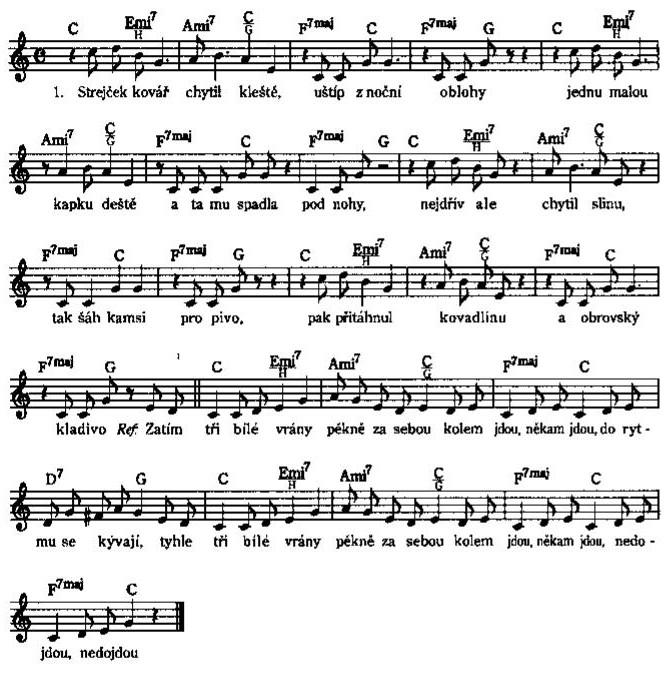
\includegraphics[width=\textwidth]{noty/a_kluziště} \end{song} \pagebreak

\setcounter{page}{43}
\begin{song}{Kometa}{C}{Jaromír Nohavica}
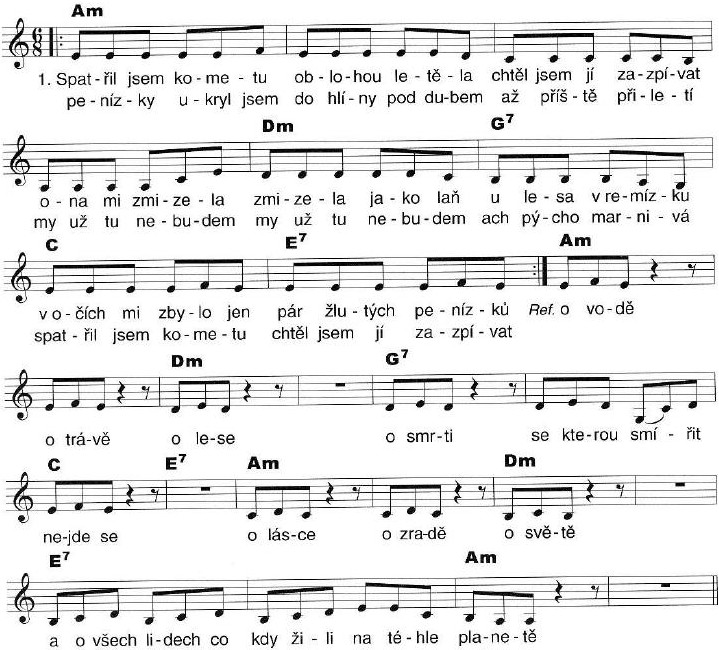
\includegraphics[width=\textwidth]{noty/a_kometa} \end{song} \pagebreak

\setcounter{page}{44}
\begin{song}{Kozel}{G}{Jaromír Nohavica}
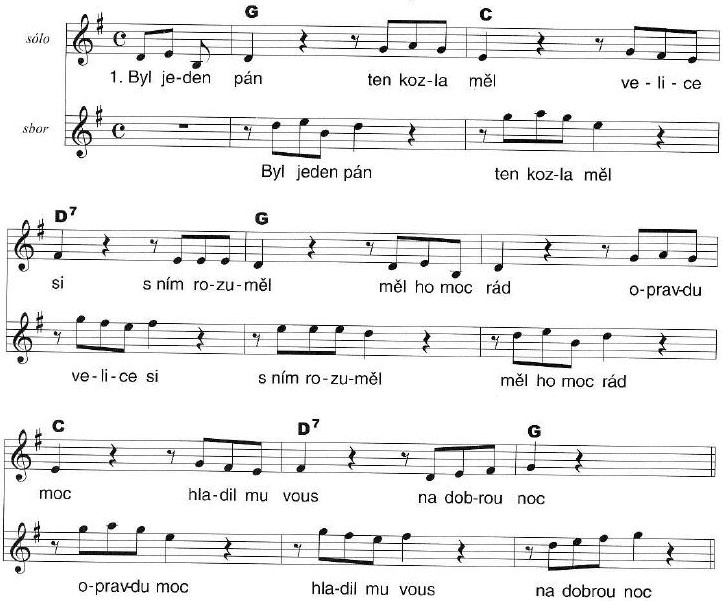
\includegraphics[width=\textwidth]{noty/a_kozel} \end{song} \pagebreak

\setcounter{page}{45}
\begin{song}{Krtek}{C}{Buty}
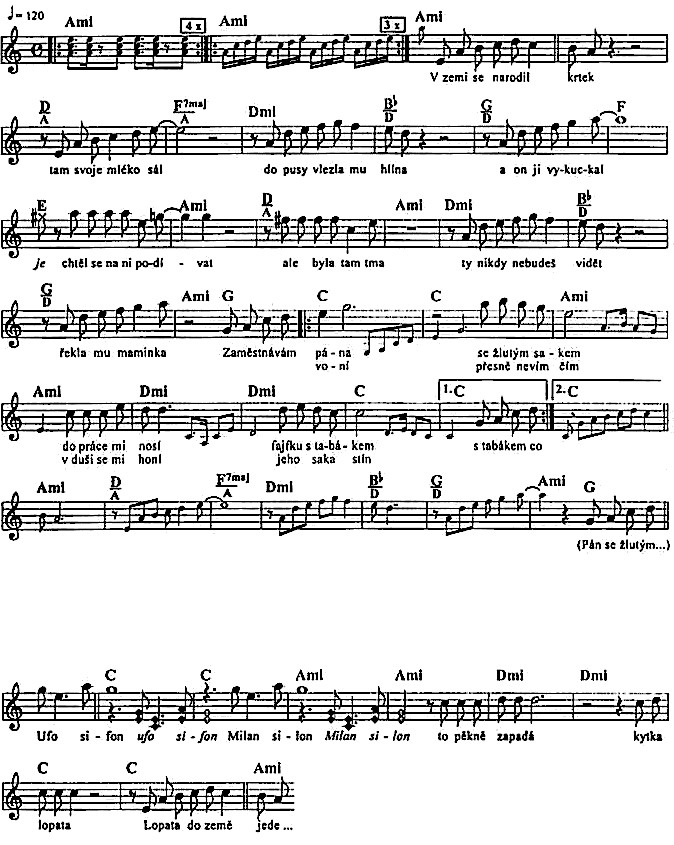
\includegraphics[width=\textwidth]{noty/a_krtek} \end{song} \pagebreak

\setcounter{page}{46}
\begin{song}{Lodníkův lament}{G}{Hop Trop}
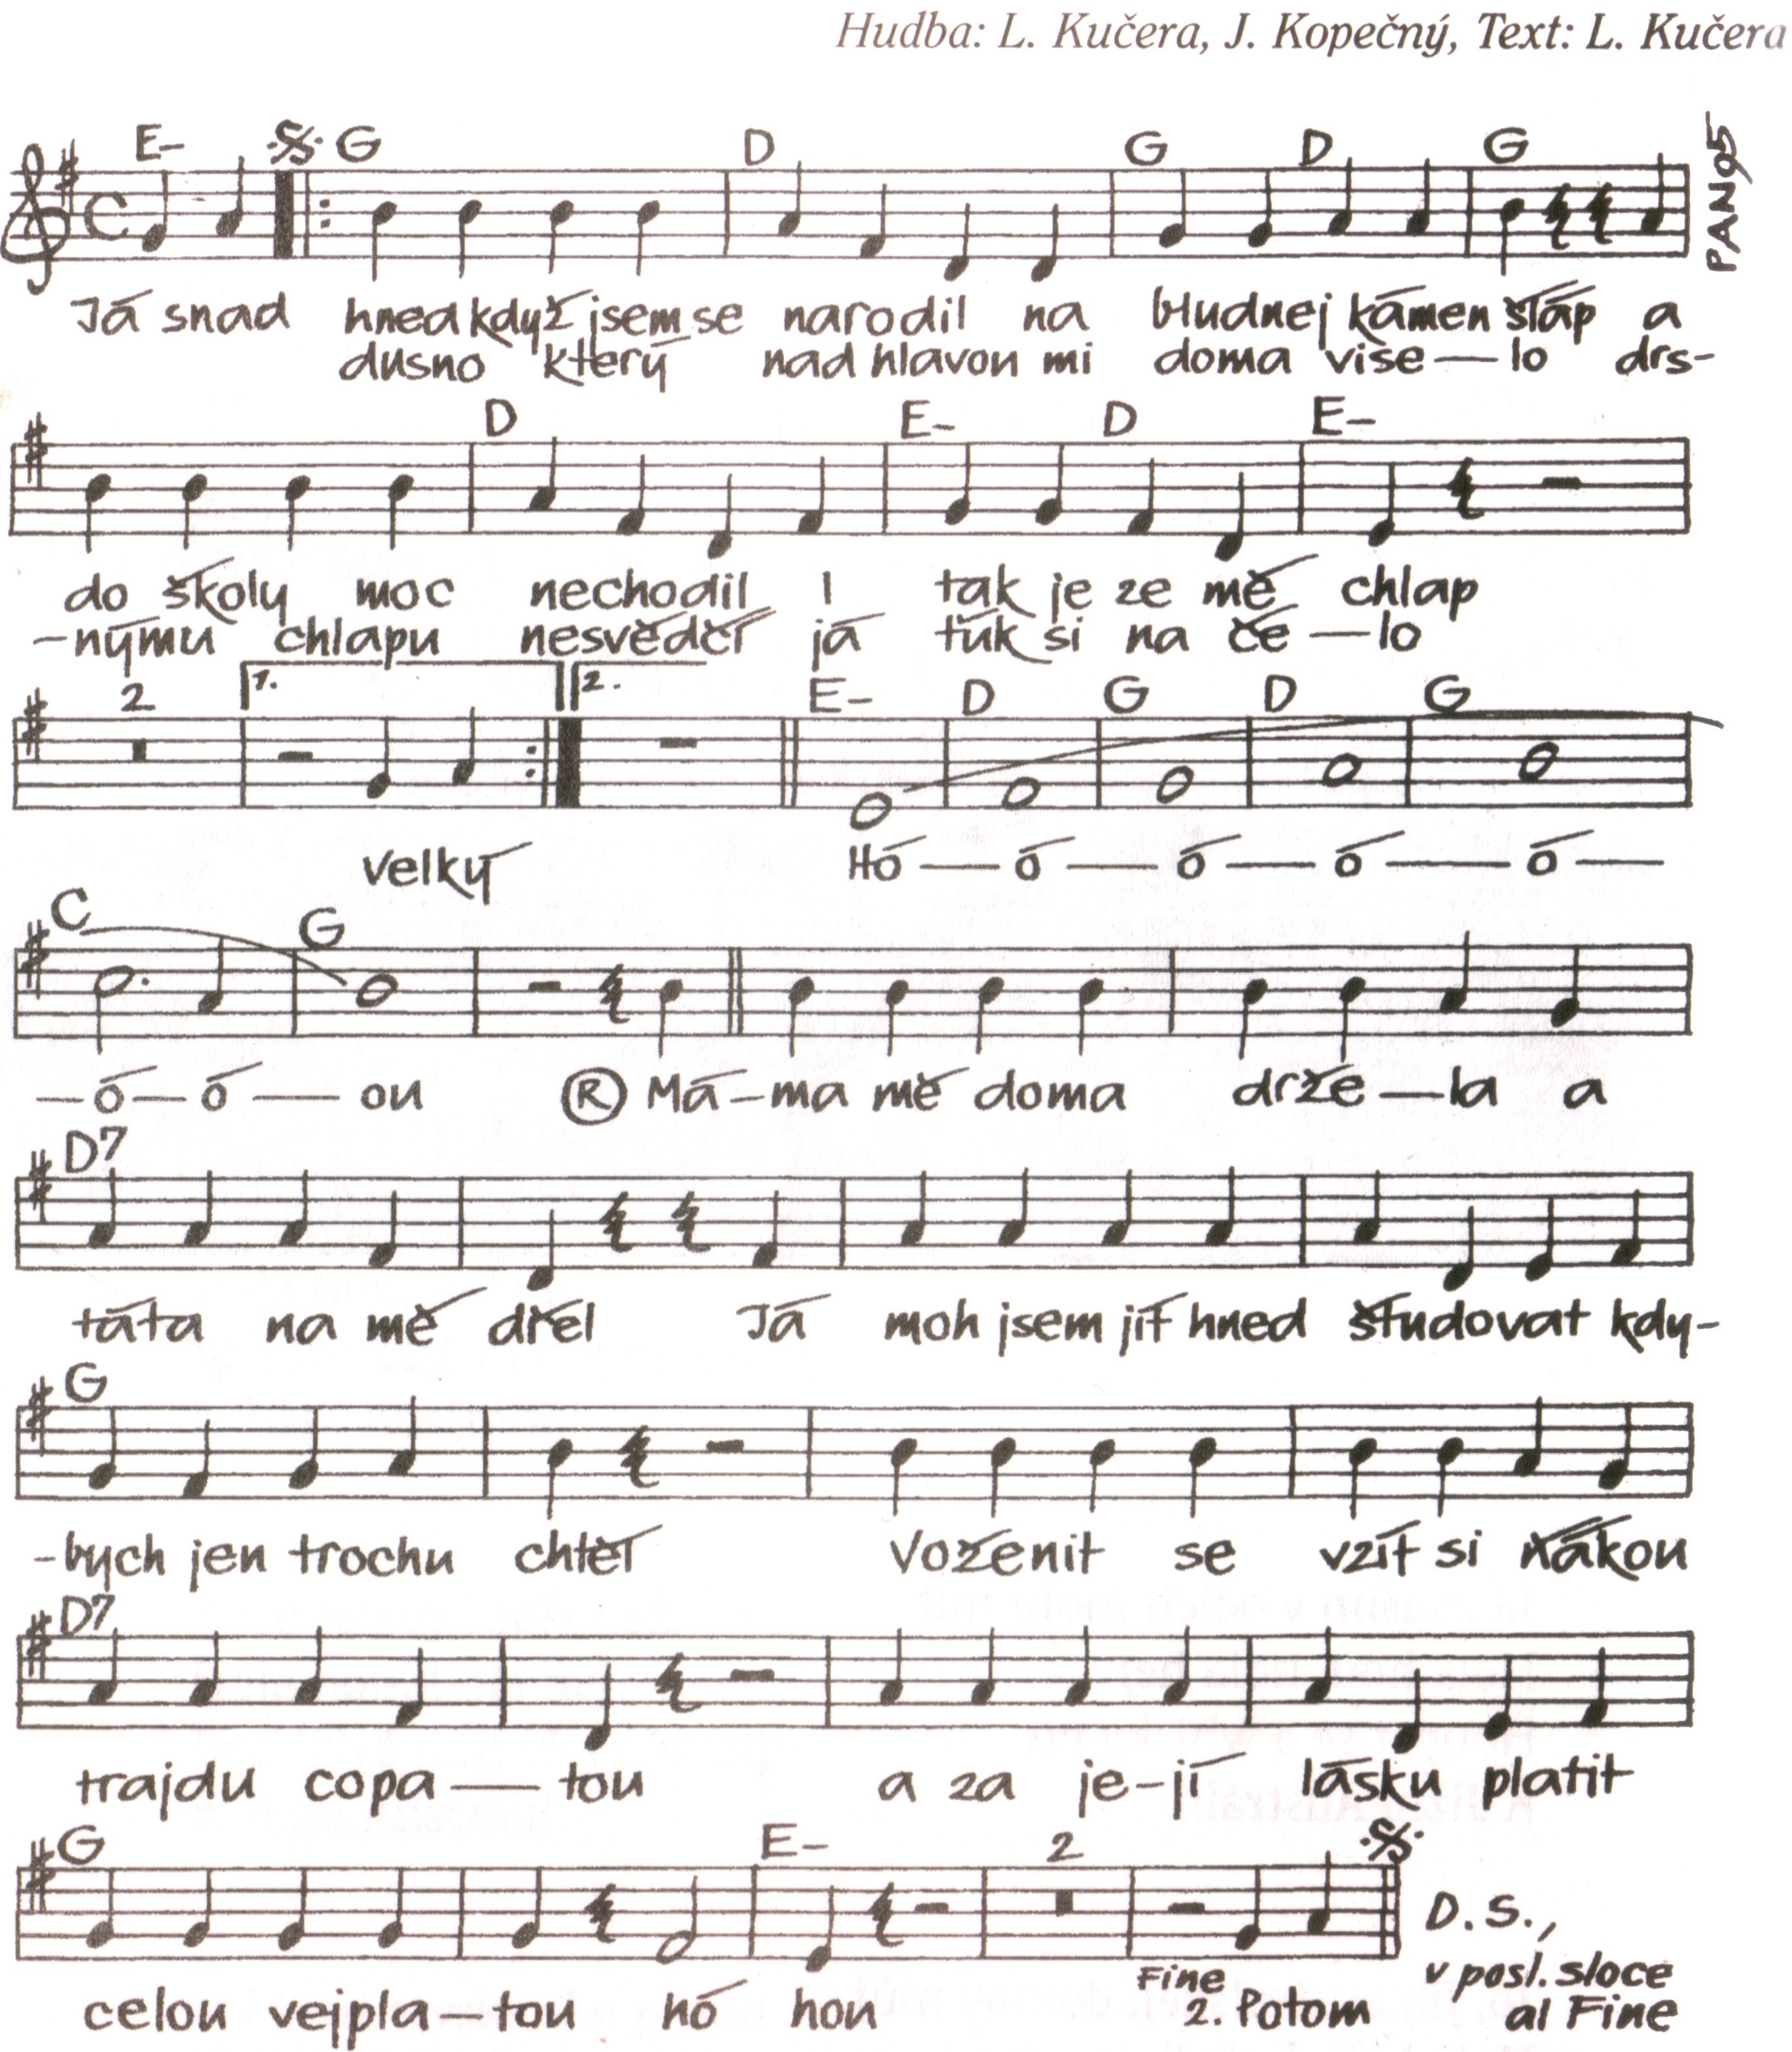
\includegraphics[width=\textwidth]{noty/a_lodníkův-lament}
\end{song}
\pagebreak

\setcounter{page}{50}
\begin{song}{Marsyas a Apollon}{G}{Marsyas}
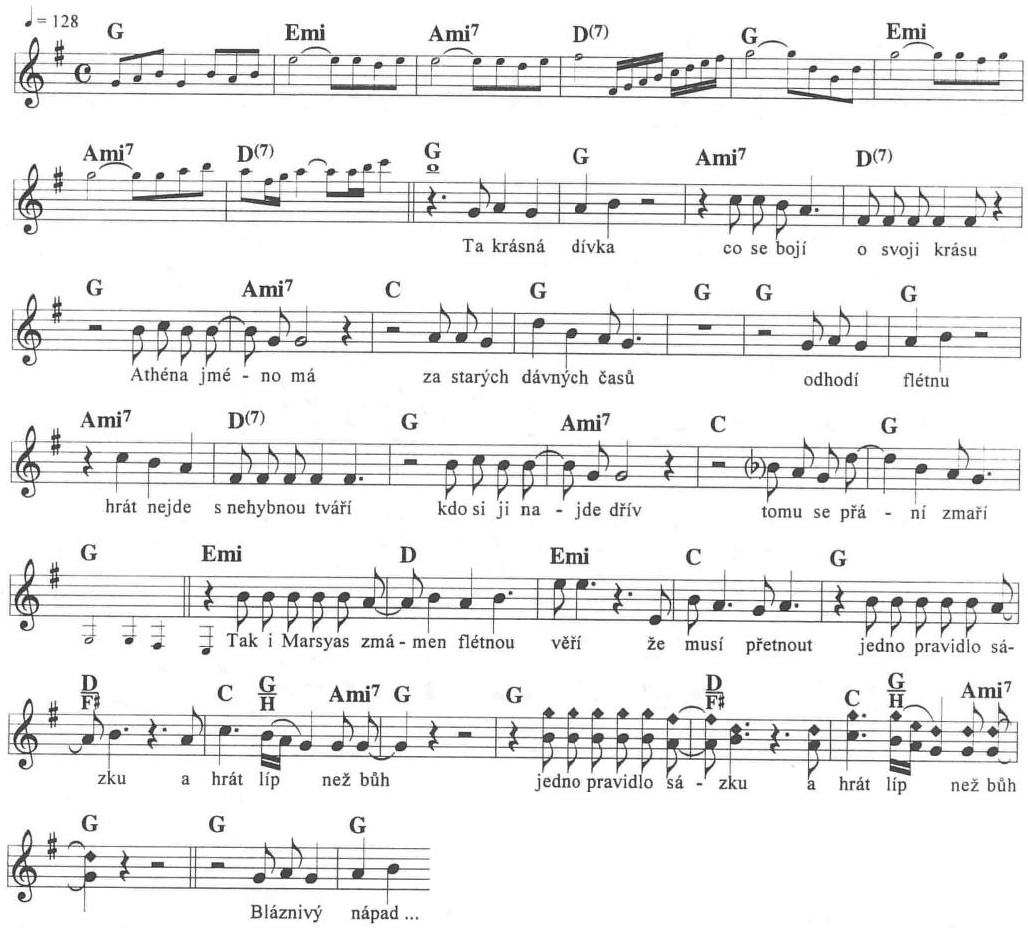
\includegraphics[width=\textwidth]{noty/a_marsyas-a-apollon} \end{song} \pagebreak

\setcounter{page}{51}
\begin{song}{Mezi horami}{F}{Čechomor}
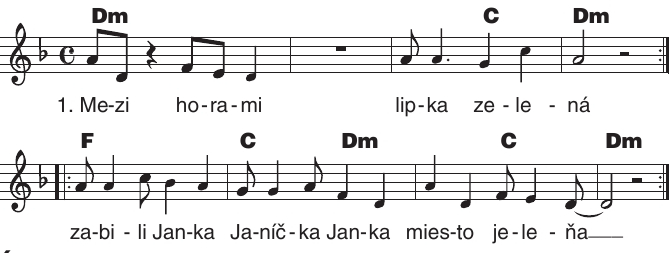
\includegraphics[width=\textwidth]{noty/a_mezi-horami} \end{song} \pagebreak

\setcounter{page}{52}
\begin{song}{Mlýny}{G}{Spirituál Kvintet}
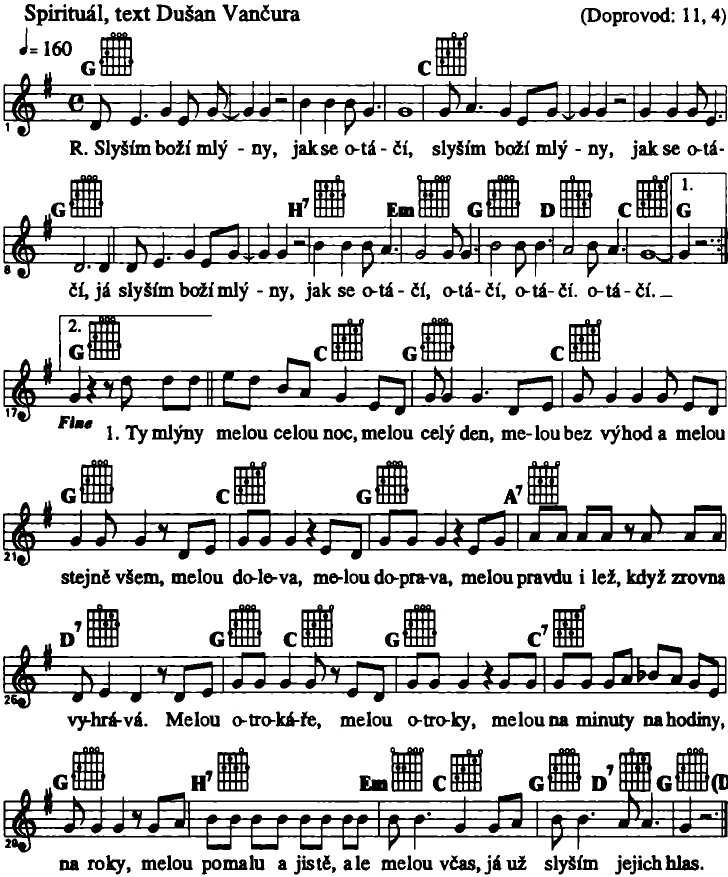
\includegraphics[width=\textwidth]{noty/a_mlýny} \end{song} \pagebreak

\setcounter{page}{53}
\begin{song}{Montgomery}{D}{}
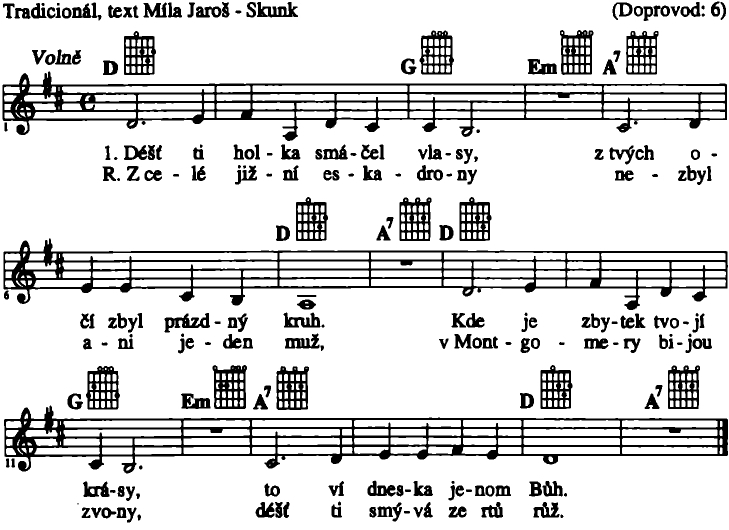
\includegraphics[width=\textwidth]{noty/a_montgomery} \end{song} \pagebreak

\setcounter{page}{54}
\begin{song}{Morituri te salutant}{C}{Karel Kryl}
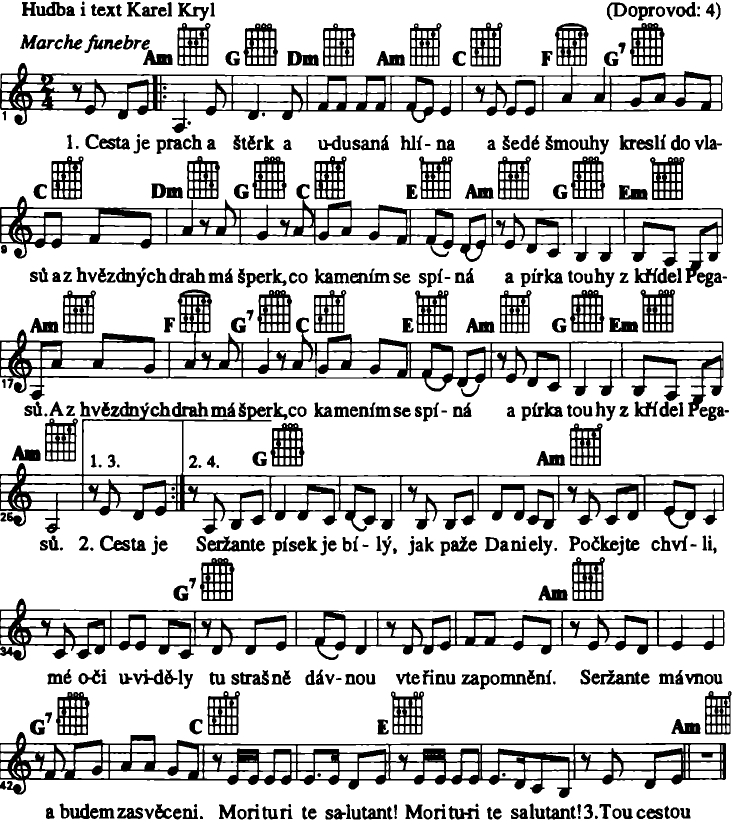
\includegraphics[width=\textwidth]{noty/a_morituri-te-salutant} \end{song} \pagebreak

\setcounter{page}{57}
\begin{song}{Nosorožec}{C}{Karel Plíhal}
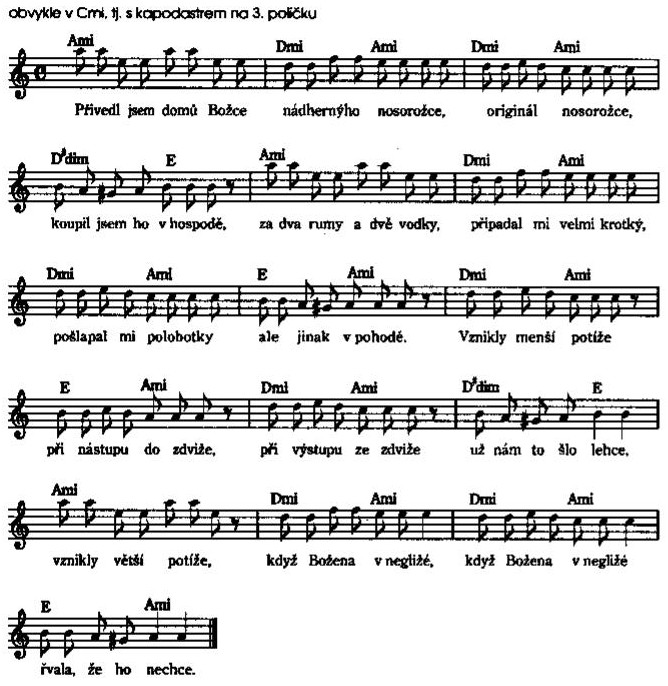
\includegraphics[width=\textwidth]{noty/a_nosorožec} \end{song} \pagebreak

\setcounter{page}{60}
\begin{song}{Ohníčky}{G}{Krausberry}
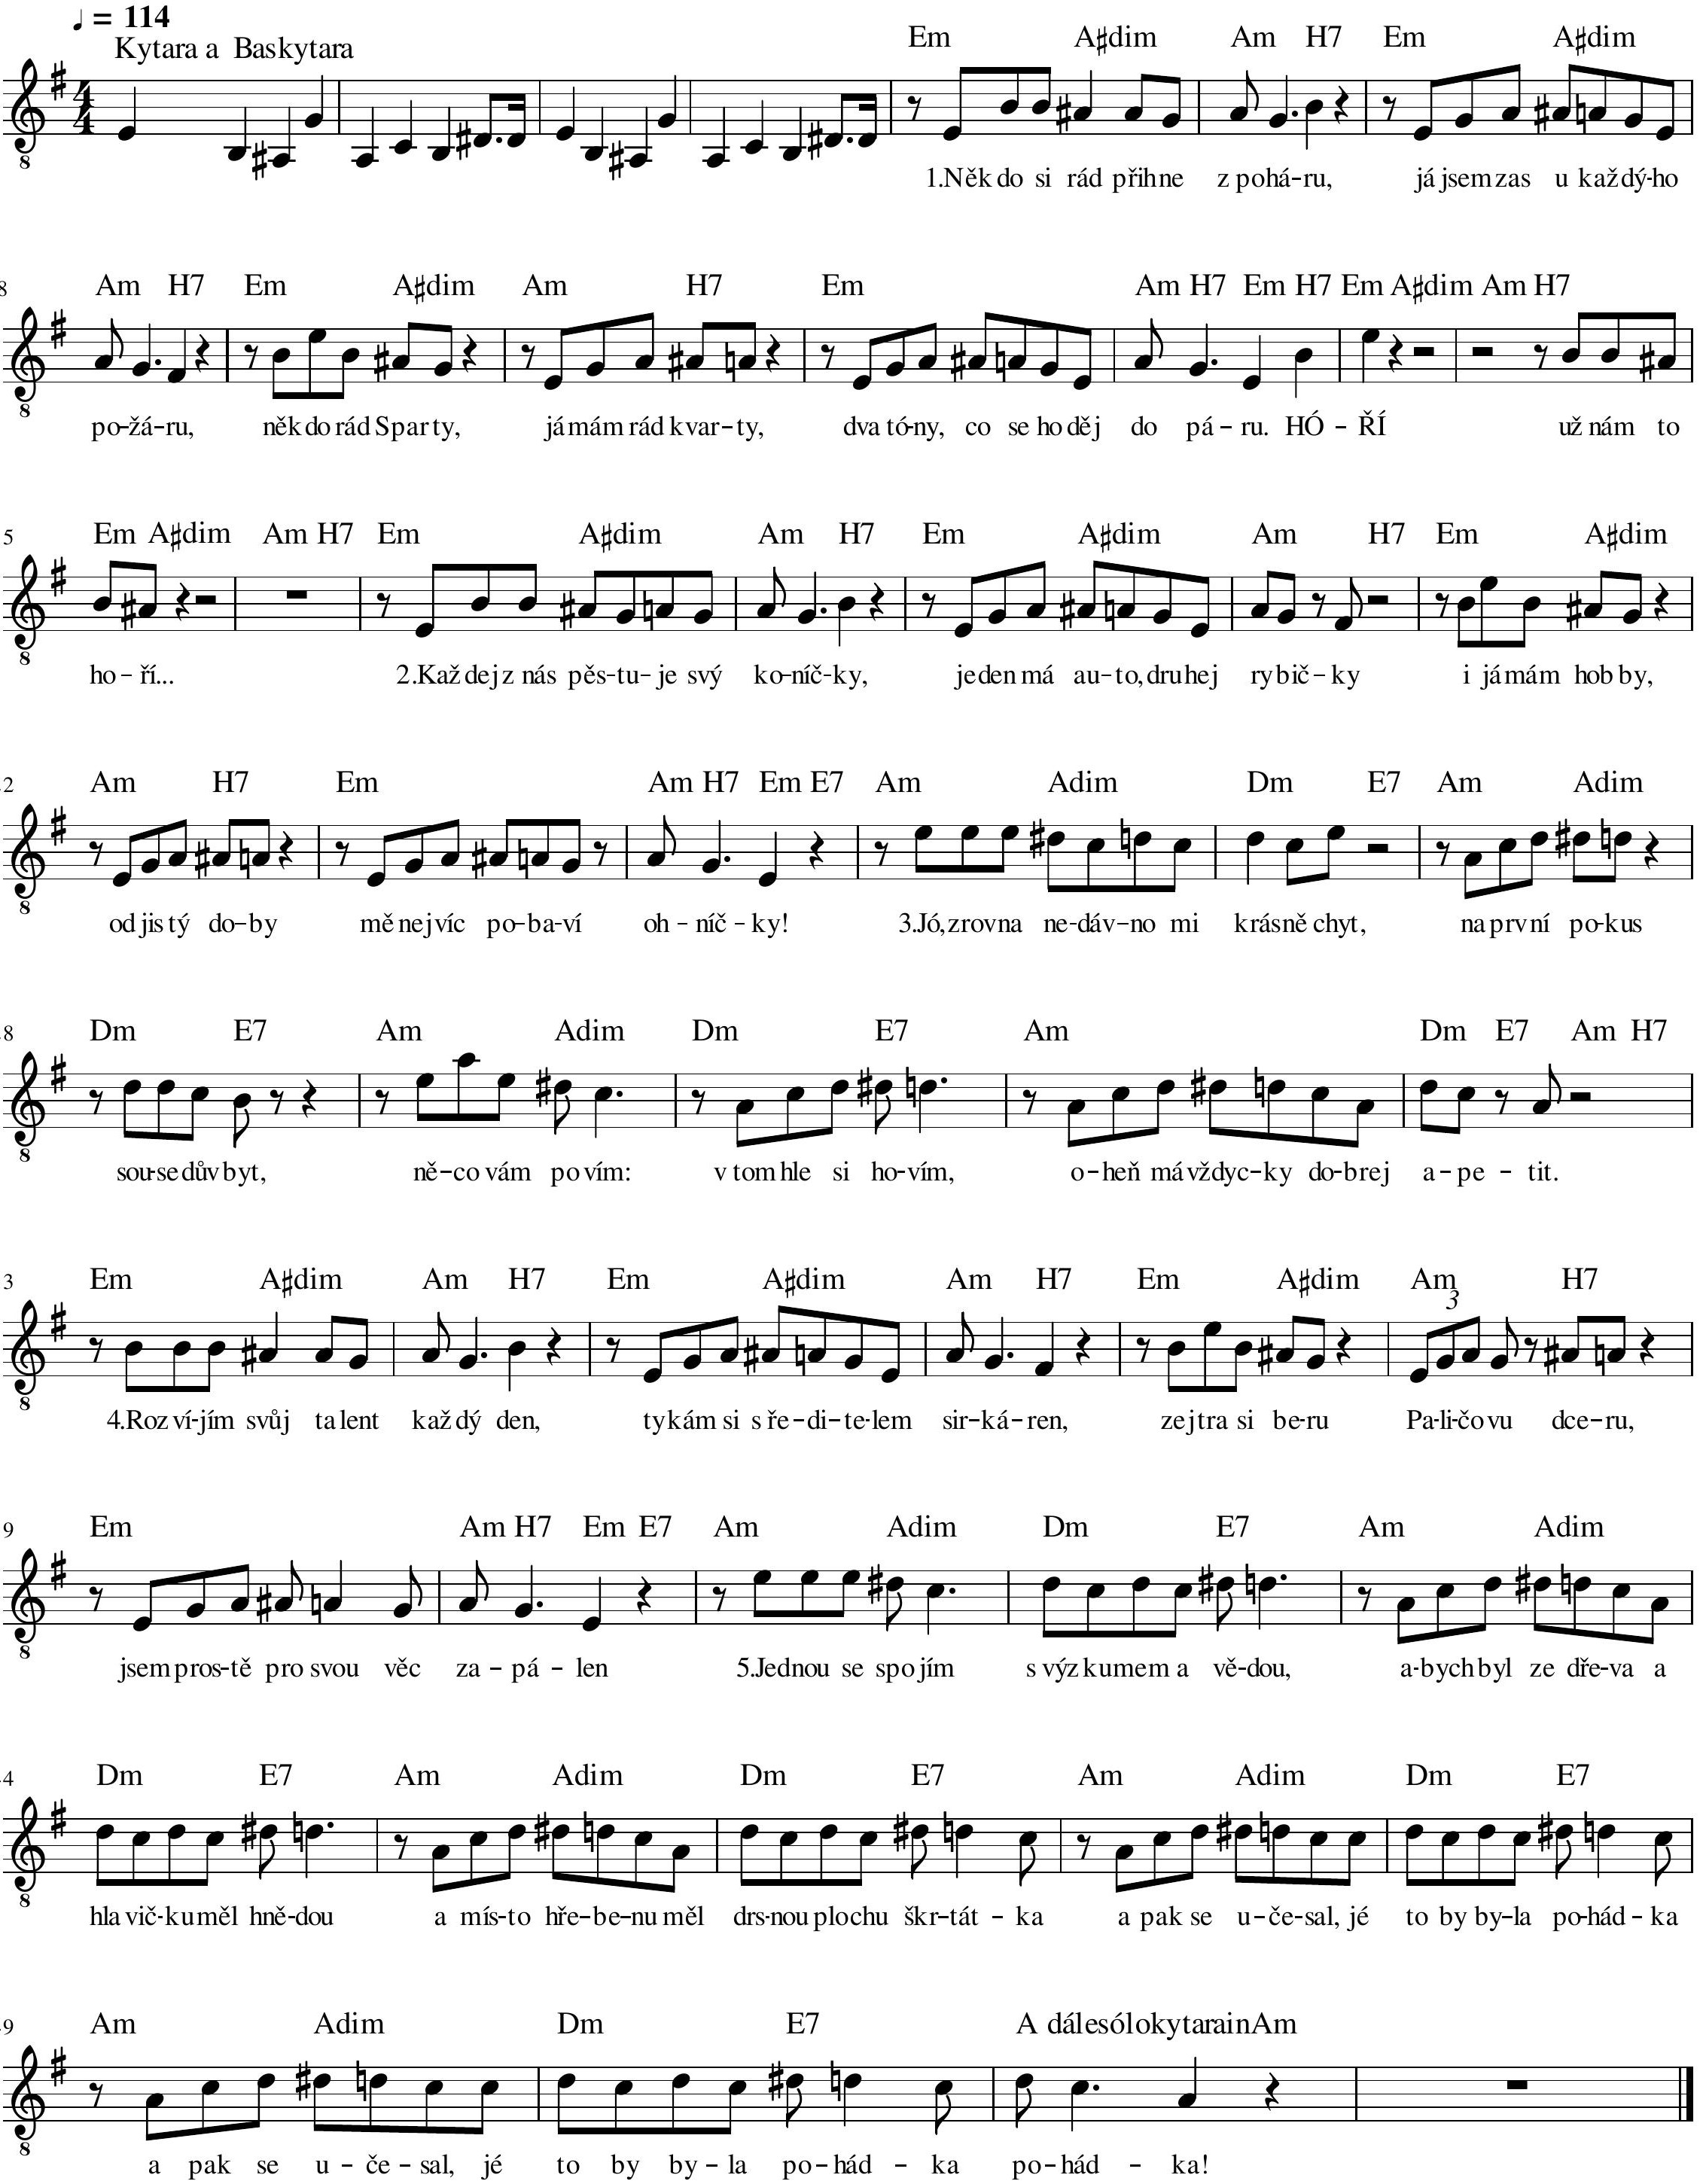
\includegraphics[width=\textwidth]{noty/a_ohníčky} \end{song} \pagebreak

\input{noty/a_o-zlaté-rybce.tex}
\setcounter{page}{64}
\begin{song}{Pánové nahoře}{C}{Jaromír Nohavica}
\begin{center}
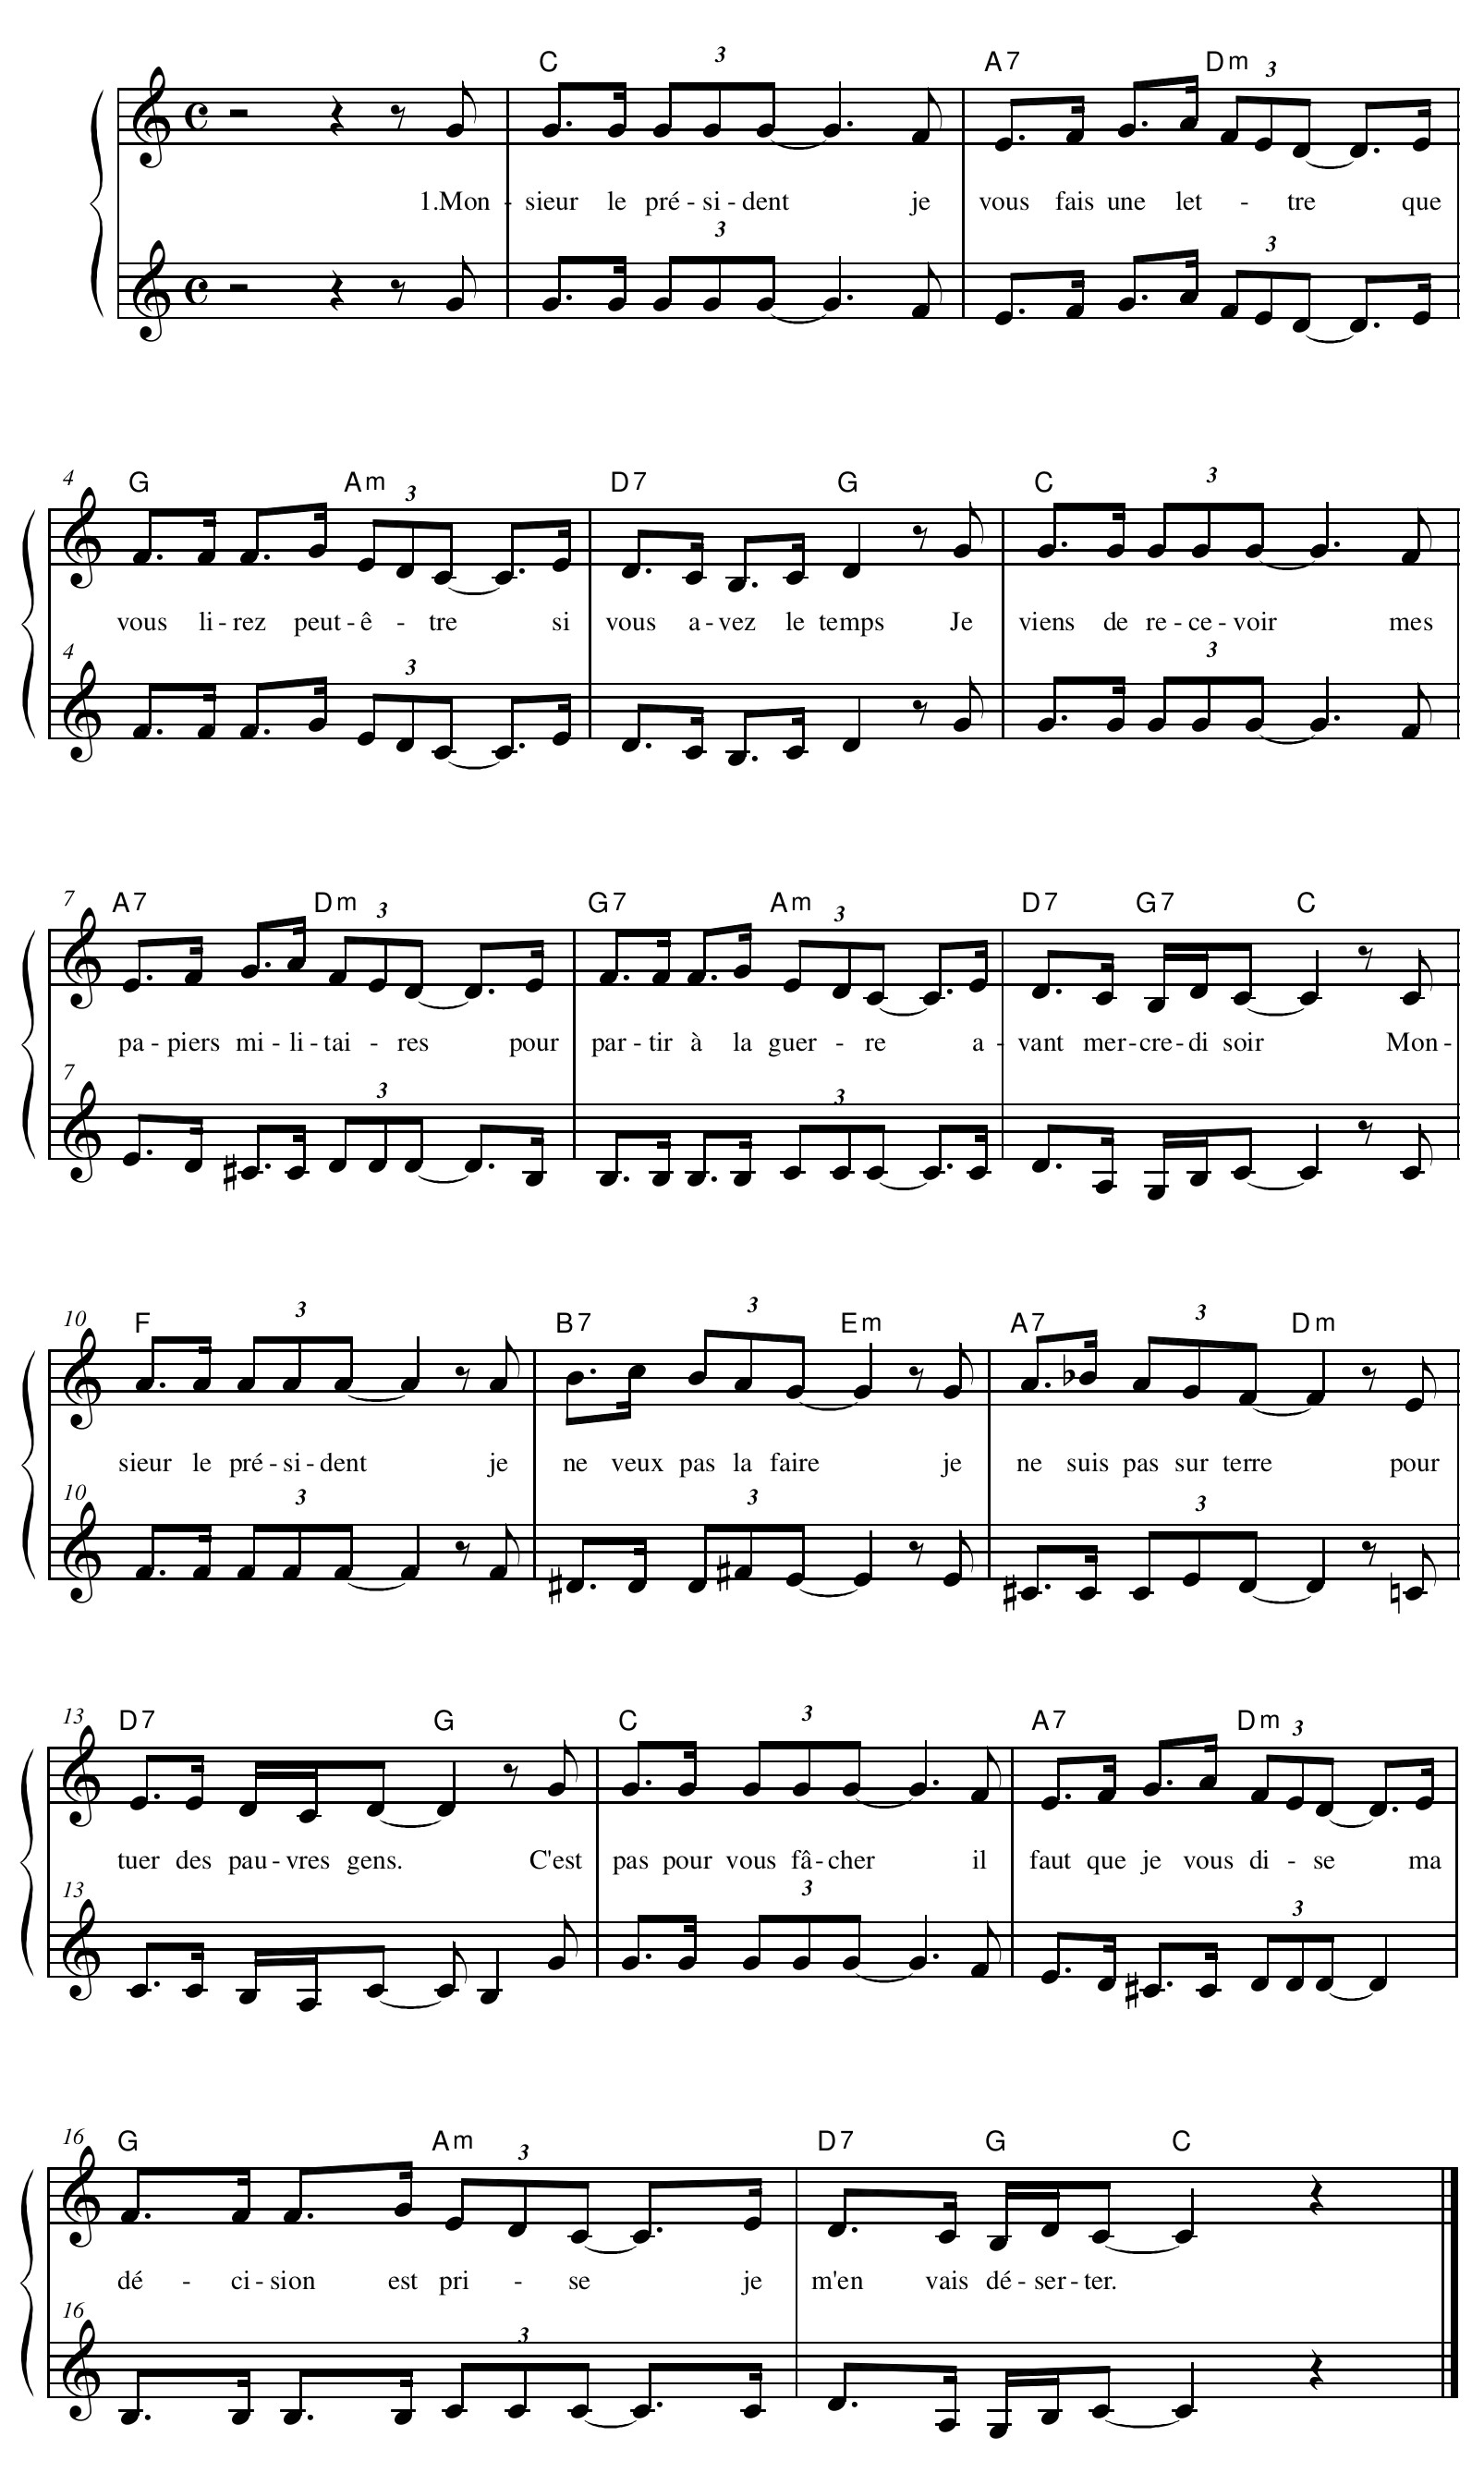
\includegraphics[height=0.9\textheight]{noty/a_pánové-nahoře} 
\end{center}
\end{song} \pagebreak

\setcounter{page}{65}
\begin{song}{Petěrburg}{C}{Jaromír Nohavica}
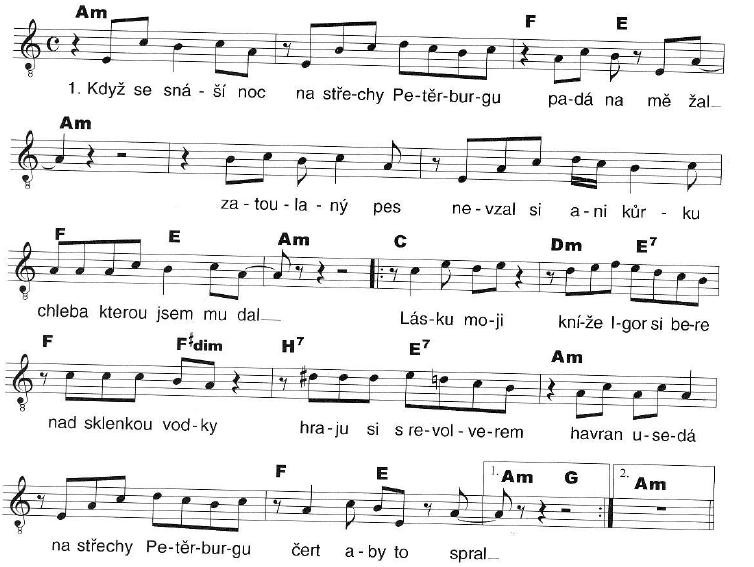
\includegraphics[width=\textwidth]{noty/a_petěnburg} \end{song} \pagebreak

\setcounter{page}{66}
\begin{song}{Pískající cikán}{G}{Spiritual kvintet}
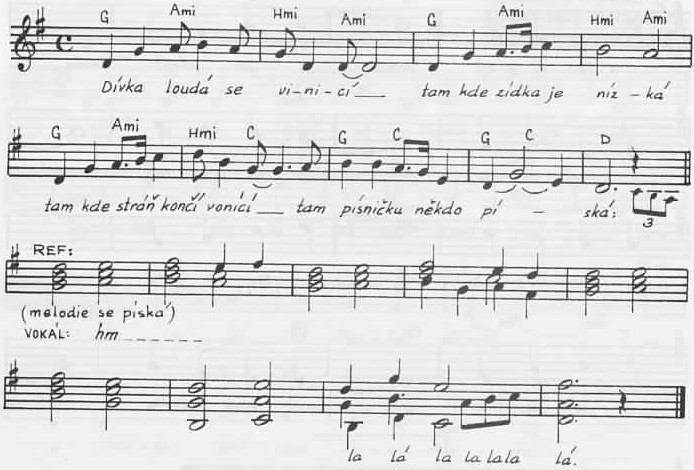
\includegraphics[width=\textwidth]{noty/a_pískající-cikán} \end{song} \pagebreak

\input{noty/a_pohár-a-kalich.tex}
\setcounter{page}{68}
\begin{song}{Pošťák}{C}{Hop Trop}\setcounter{page}{68} 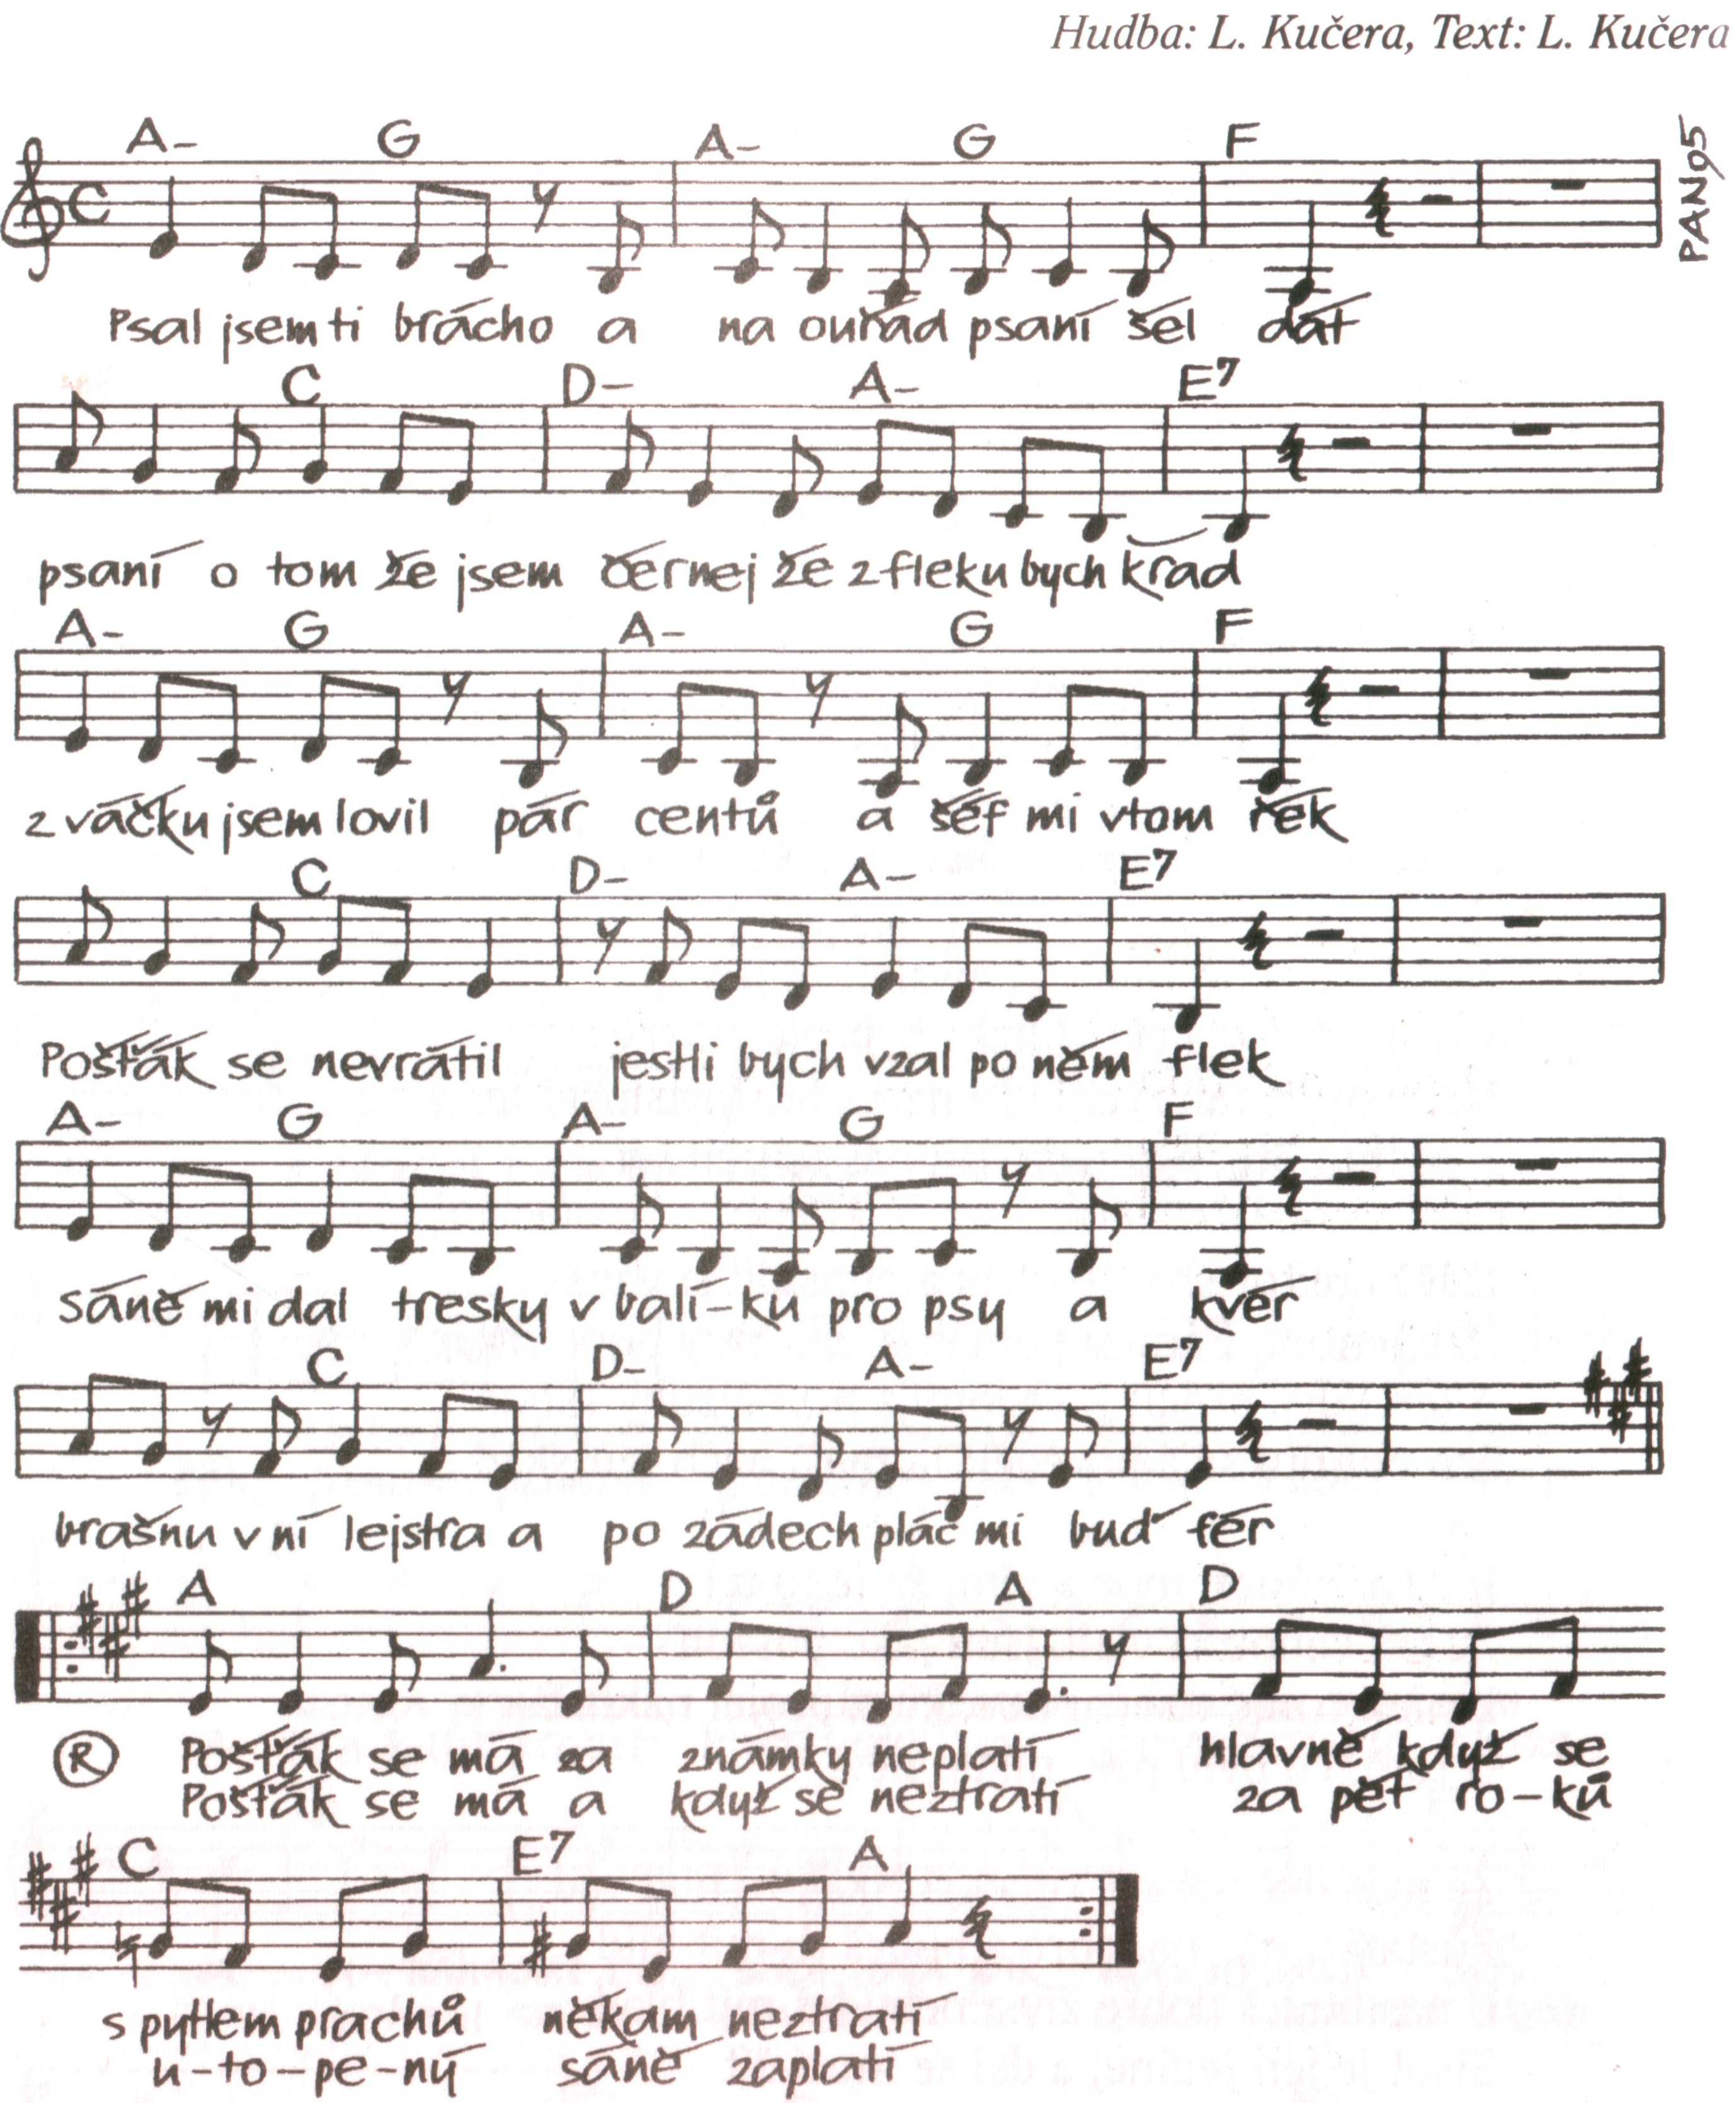
\includegraphics[width=\textwidth]{noty/a_pošťák}
\end{song} \pagebreak

\setcounter{page}{69}
\begin{song}{Pověste ho vejš}{G}{Michal Tučný}
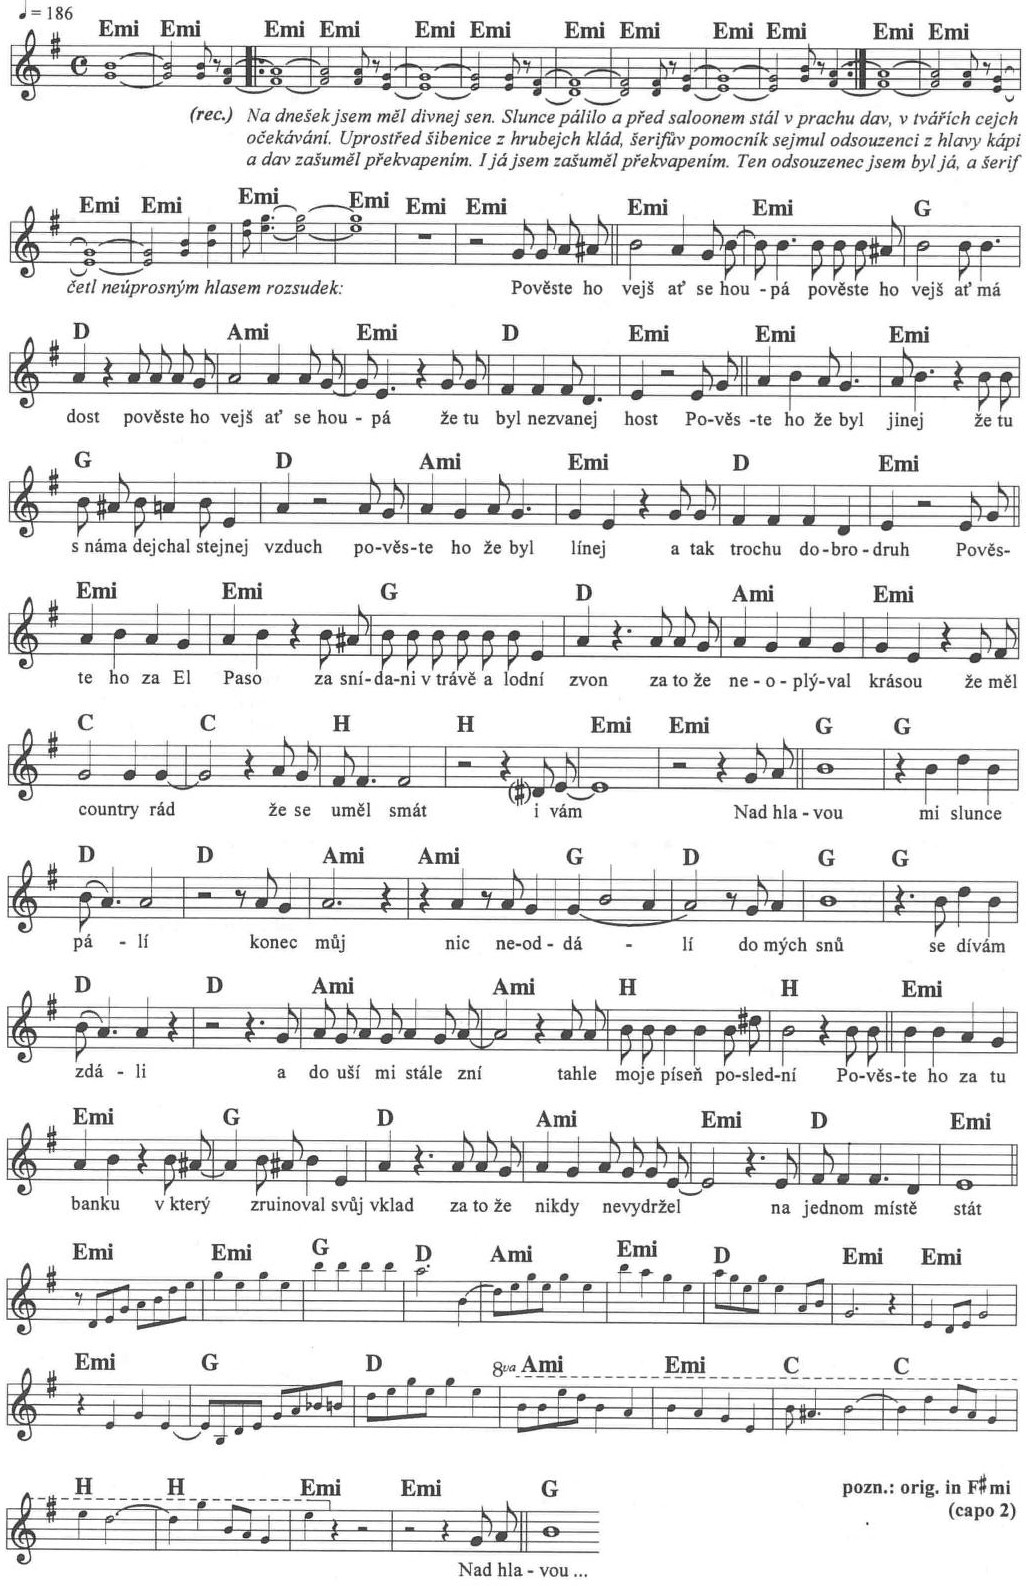
\includegraphics[width=\textwidth]{noty/a_pověste-ho-vejš} \end{song} \pagebreak

\setcounter{page}{70}
\begin{song}{Prasátko}{G}{Buty}
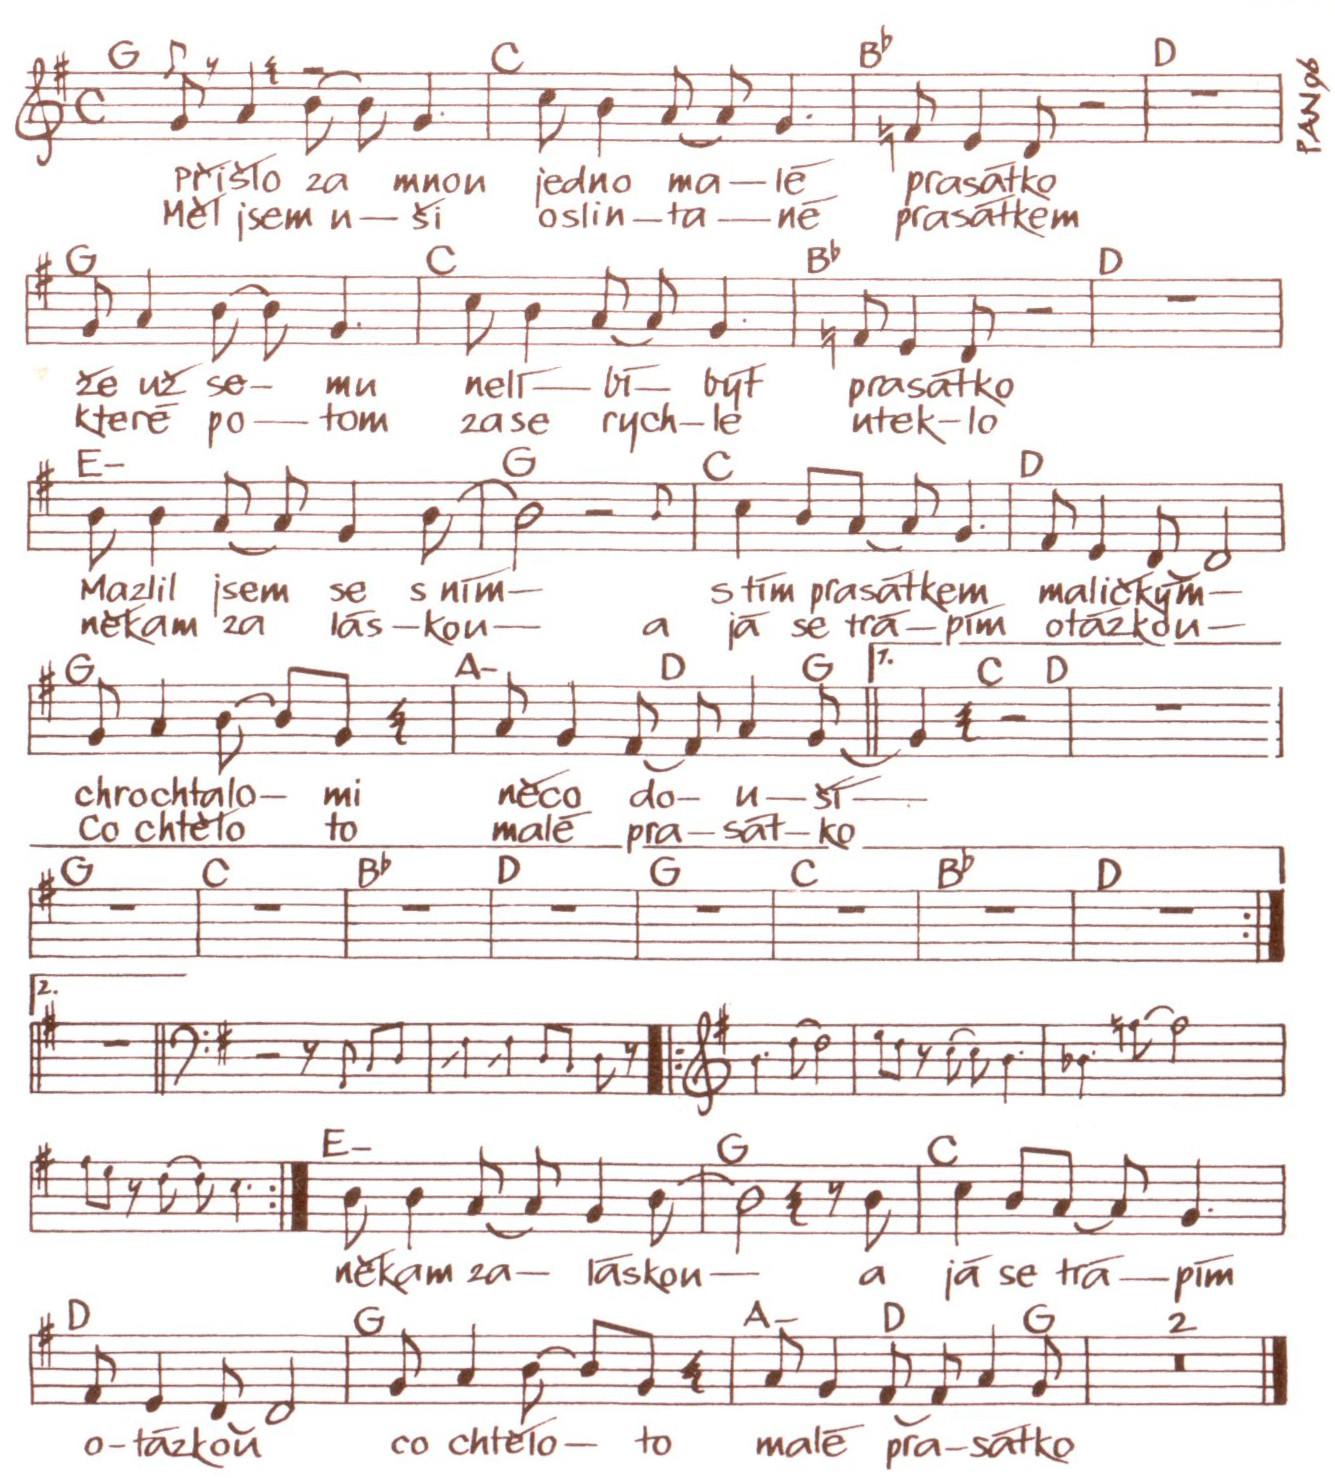
\includegraphics[width=\textwidth]{noty/a_prasátko} \end{song} \pagebreak

\setcounter{page}{71}
\begin{song}{Prší}{C}{Karel Plíhal}
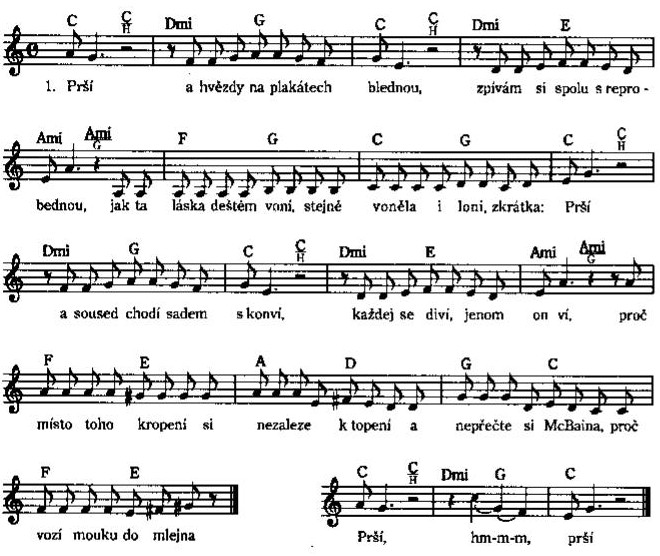
\includegraphics[width=\textwidth]{noty/a_prší} \end{song} \pagebreak

\input{noty/a_ráda-se-miluje.tex}
\setcounter{page}{73}
\begin{song}{Rána v trávě}{C}{Žalman}
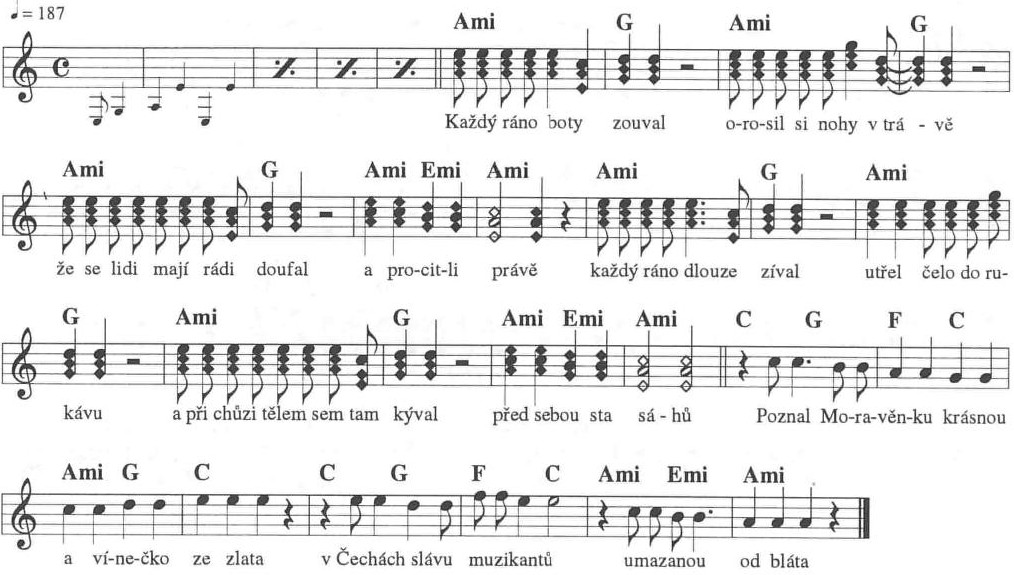
\includegraphics[width=\textwidth]{noty/a_rána-v-trávě} \end{song} \pagebreak

\input{noty/a_rosa-na-kolejích.tex}
\setcounter{page}{75}
\begin{song}{Růže z papíru}{F}{Brontosauři}
\includegraphics[width=\textwidth]{noty/a_růže-z-papíru} \end{song} \pagebreak

\setcounter{page}{76}
\begin{song}{Ryl jen, celej den ryl}{Es}{Spiritual kvintet}
\includegraphics[width=\textwidth]{noty/a_ryl-jen-celej-den-ryl} \end{song} \pagebreak

\setcounter{page}{77}
\begin{song}{Sáro}{C}{Traband}
\includegraphics[width=\textwidth]{noty/a_sáro} \end{song} \pagebreak

\setcounter{page}{78}
\begin{song}{Severní vítr}{D}{Zdeněk Svěrák a Jaroslav Uhlíř}
 \includegraphics[width=\textwidth]{noty/a_severní-vítr} \end{song}\pagebreak

\input{noty/a_slavíci-z-madridu.tex}
\input{noty/a_soudný-den.tex}
\setcounter{page}{83}
\begin{song}{Stýskání}{D}{Bratři Ebenové}
\setcounter{page}{83} \includegraphics[width=\textwidth]{noty/a_styskani} 
\end{song}
\pagebreak

\setcounter{page}{84}
\begin{song}{Tak už mi má holka mává}{G}{Hoboes}
\begin{center}
\includegraphics[height=0.9\textheight]{noty/a_tak-už-mi-má-holka-mává} 
\end{center}
\end{song} \pagebreak

\setcounter{page}{85}
\begin{song}{Tereza}{G}{Wabi Ryvola}
\begin{center}
\includegraphics[width=0.8\textwidth]{noty/a_tereza} 
\end{center}
\end{song} \pagebreak

\setcounter{page}{86}
\begin{song}{Těšínská}{C}{Jaromír Nohavica}
\includegraphics[width=\textwidth]{noty/a_těšínská} \end{song} \pagebreak

\setcounter{page}{87}
\begin{song}{Tisíc dnů mezi námi}{C}{Nerez}
\begin{center}
\includegraphics[height=0.9\textheight]{noty/a_tisíc-dnů-mezi-námi} 
\end{center}
\end{song} \pagebreak

\setcounter{page}{88}
\begin{song}{Topič}{C}{Karel Plíhal}

\includegraphics[width=\textwidth]{noty/a_topič} \end{song} \pagebreak

\setcounter{page}{90}
\begin{song}{To ta Heľpa}{F}{Tradicionál (sk)}
\includegraphics[width=\textwidth]{noty/a_to-ta-helpa} \end{song} \pagebreak

\setcounter{page}{91}
\begin{song}{Toulavej}{C}{Vojtěch 'Kiďák' Tomáško}
\includegraphics[width=\textwidth]{noty/a_toulavej} \end{song} \pagebreak

\setcounter{page}{92}
\begin{song}{Trampská}{F}{Bratři Ebenové}
\setcounter{page}{92} \includegraphics[width=\textwidth]{noty/a_trampská} 
\end{song}
\pagebreak

\setcounter{page}{93}
\begin{song}{Tři kříže}{F}{Hop trop}
\setcounter{page}{93} \includegraphics[width=\textwidth]{noty/a_tři-kříže} 
\end{song}
\pagebreak

\setcounter{page}{94}
\begin{song}{Tulácký ráno}{F}{Jan Nedvěd}
\includegraphics[width=\textwidth]{noty/a_tulácký-ráno} \end{song} \pagebreak

\setcounter{page}{95}
\begin{song}{Už to nenapravím}{C}{Jaroslav Samson Lenk}
\includegraphics[width=\textwidth]{noty/a_už-to-nenapravím} \end{song} \pagebreak

\setcounter{page}{96}
\begin{song}{Válka růží}{F}{Spiritual Kvintet}
\includegraphics[width=\textwidth]{noty/a_válka-růží} \end{song} \pagebreak

\setcounter{page}{97}
\begin{song}{Velrybářská výprava}{C}{Antonín Linhart}
\includegraphics[width=\textwidth]{noty/a_velrybářská-výprava} \end{song} \pagebreak

\setcounter{page}{98}
\begin{song}{Vlajka}{F,D}{Jan Korda}
\includegraphics[width=\textwidth]{noty/a_vlajka} \end{song} \pagebreak

\input{noty/a_vstávej-holka.tex}
\setcounter{page}{100}
\begin{song}{Zabili, zabili}{D}{Tradicionál}
\includegraphics[width=\textwidth]{noty/a_zabili-zabili} \end{song} \pagebreak

\setcounter{page}{101}
\begin{song}{Zafúkané}{C}{Fleret}
\includegraphics[width=\textwidth]{noty/a_zafúkané} \end{song} \pagebreak

\setcounter{page}{102}
\begin{song}{Zatanči}{G}{Jaromír Nohavica}
\includegraphics[width=\textwidth]{noty/a_zatanči} \end{song} \pagebreak

\setcounter{page}{103}
\begin{song}{Zítra ráno v pět}{G}{Jaromír Nohavica}
\includegraphics[width=\textwidth]{noty/a_zítra-ráno-v-pět} \end{song} \pagebreak

\section{Rybičkovky}

\begin{multicols}{2}

\setcounter{page}{104}
\begin{song}{Apoštolská}{G}{}
\includegraphics[width=0.5\textwidth]{noty/b_Apoštolská} \end{song}

\setcounter{page}{104}
\begin{song}{Boží radost jak řeka}{G}{}
\includegraphics[width=0.5\textwidth]{noty/b_Boží-radost-jako-řeka} \end{song}
\columnbreak

\setcounter{page}{105}
\begin{song}{Bůh je záštita má}{G}{}
\includegraphics[width=0.5\textwidth]{noty/b_Bůh-je-záštita-má} \end{song}

\setcounter{page}{105}
\begin{song}{Effatha}{G}{}
\includegraphics[width=0.5\textwidth]{noty/b_Effatha} \end{song}
\pagebreak

\setcounter{page}{105}
\begin{song}{Hosana}{G}{}
\includegraphics[width=0.5\textwidth]{noty/b_Hosana} \end{song}

\setcounter{page}{106}
\begin{song}{Jsem všechno, co nemáš}{D}{}
\includegraphics[width=0.45\textwidth]{noty/b_Jsem-všechno-co-nemáš} \end{song}

\setcounter{page}{107}
\begin{song}{Laudato Sii}{E}{}
\includegraphics[width=0.5\textwidth]{noty/b_Laudato-si} \end{song}

\setcounter{page}{107}
\begin{song}{Modlitba sv. Tomáše Mora}{A}{}
\includegraphics[width=0.5\textwidth]{noty/b_Modlitba-sv-Tomáše} \end{song}

\setcounter{page}{108}
\begin{song}{Na Golgotu}{D}{}
\includegraphics[width=0.45\textwidth]{noty/b_Na-Golgotu} \end{song}
\pagebreak

\setcounter{page}{109}
\begin{song}{Nám, Pane, dal jsi slovo své}{F}{}
\includegraphics[width=0.5\textwidth]{noty/b_Nám-pane-dal-jsi-slovo-své} \end{song}

\setcounter{page}{109}
\begin{song}{Neseme, Pane, chléb a víno}{F}{}
\includegraphics[width=0.5\textwidth]{noty/b_Neseme-pane-chléb-a-víno} \end{song}

\setcounter{page}{110}
\begin{song}{Ó, Pane, zhasíná den}{E}{}
\includegraphics[width=0.5\textwidth]{noty/b_Ó-pane-zhasíná-den} \end{song}

\setcounter{page}{110}
\begin{song}{Pojď ke mně blíž}{G}{}
\includegraphics[width=0.5\textwidth]{noty/b_oPojď-ke-mně-blíž} \end{song}
\pagebreak

\setcounter{page}{111}
\begin{song}{Ordinarium IV}{CDGAC}{}
\subsubsection*{KYRIE}
\includegraphics[width=0.5\textwidth]{noty/c_o4-kyrie} 
\subsubsection*{GLORIA}
\includegraphics[width=0.5\textwidth]{noty/c_o4-gloria} 
\columnbreak
\subsubsection*{CREDO}
\includegraphics[width=0.5\textwidth]{noty/c_o4-credo} 
\subsubsection*{SANCTUS}
\includegraphics[width=0.5\textwidth]{noty/c_o4-sanctus}
\subsubsection*{AGNUS DEI}
\includegraphics[width=0.5\textwidth]{noty/c_o4-agnus-dei} 

\end{song}
\pagebreak

\setcounter{page}{112}
\begin{song}{Pojďte ke mě všichni}{D}{}
\includegraphics[width=0.5\textwidth]{noty/b_Pojďte-ke-mně-všichni} \end{song}

\input{noty/b_Posba-k-Duchu-svatému.tex}
\setcounter{page}{113}
\begin{song}{Příjmám}{D}{}
\includegraphics[width=0.5\textwidth]{noty/b_Prijímám} \end{song}

\setcounter{page}{114}
\begin{song}{Přijmi, Pane}{G}{}
\includegraphics[width=0.5\textwidth]{noty/b_Prijmi-pane} \end{song}
\pagebreak


\input{noty/b_Připravujte-cestu.tex}
\setcounter{page}{121}
\begin{song}{Zde jsem}{E}{}
\includegraphics[width=0.41\textwidth]{noty/b_Zde-jsem} \end{song}

\end{multicols}
\setcounter{page}{116}
\begin{song}{Půjdeš-li pouští}{C}{}
\includegraphics[width=\textwidth]{noty/b_Půjdeš-li-pouští} \end{song}
\begin{multicols}{2}

\input{noty/b_Slunce-kristovy-lásky.tex}
\input{noty/b_Spoj-nás-v-jedno.tex}
\setcounter{page}{117}
\begin{song}{Světem běžím dál}{C}{}
\includegraphics[width=0.5\textwidth]{noty/b_Světem-běžím-dál} \end{song}

\setcounter{page}{117}
\begin{song}{Svorni jsme}{G}{}
\includegraphics[width=0.5\textwidth]{noty/b_Svorni-jsme} \end{song}
\pagebreak

\setcounter{page}{118}
\begin{song}{Svý kroky rozezpívej}{F}{}
\includegraphics[width=0.44\textwidth]{noty/b_Svý-kroky-rozezpívej} \end{song}



\setcounter{page}{119}
\begin{song}{Tobě patří chvála}{D}{}
\includegraphics[width=0.45\textwidth]{noty/b_Tobě-patří-chvála} \end{song}

\setcounter{page}{118}
\begin{song}{Vše, co mohu dát, je chvála}{D}{}
\includegraphics[width=0.45\textwidth]{noty/b_Vše-co-mohu-dát} \end{song}

\setcounter{page}{119}
\begin{song}{Vychází}{C}{}
\includegraphics[width=0.48\textwidth]{noty/b_Vychází} \end{song}
\clearpage

\end{multicols}
\pagebreak
\section{Zahraniční}

\setcounter{page}{126}
\begin{song}{Take me home, country roads}{D}{John Denver}
\includegraphics[width=\textwidth]{noty/c_take-me-home-country-roads} \end{song} \pagebreak

\setcounter{page}{128}
\begin{song}{The House of the Rising Sun}{F}{}
\includegraphics[width=\textwidth]{noty/c_the-house-of-the-rising-sun} \end{song} \pagebreak


\clearpage

\begin{center}
\section{Přehled akordů}
\includegraphics[width=\textwidth]{noty/akordy} 
\end{center}
\clearpage

\begin{center}
\section{Přehled rytmů}
\includegraphics[width=\textwidth]{noty/rytmy} 
\end{center}
\clearpage

\end{document}
